%%%%%%%%%%%%%%%%%%%%%%%%%%%%%%%%%%%%%%%%%%%%%%%
%
% Template per Elaborato di Laurea
% DISI - Dipartimento di Ingegneria e Scienza dell’Informazione
%
% update 2015-09-10
%
% Per la generazione corretta del 
% pdflatex nome_file.tex
% bibtex nome_file.aux
% pdflatex nome_file.tex
% pdflatex nome_file.tex
%
%%%%%%%%%%%%%%%%%%%%%%%%%%%%%%%%%%%%%%%%%%%%%%%

% formato FRONTE RETRO
\documentclass[epsfig,a4paper,11pt,titlepage,twoside,openany]{book}
\usepackage{epsfig}
\usepackage{plain}
\usepackage{cite}
\usepackage{setspace}
\usepackage[paperheight=29.7cm,paperwidth=21cm,outer=1.5cm,inner=2.5cm,top=2cm,bottom=2cm]{geometry} % per definizione layout
\usepackage{titlesec} % per formato custom dei titoli dei capitoli
\usepackage[strings]{underscore} % evita errori di bibtex in caso di caratteri underscore
\usepackage{amsfonts} % mathbb
\usepackage{amsmath} % align environment
\usepackage{bm} % bold mathematical symbols
\usepackage{graphicx} % images
\graphicspath{{graphs/}} % images global path
\usepackage{enumitem}
\usepackage[table,xcdraw]{xcolor}
\usepackage{adjustbox}
\setlength{\parindent}{0pt} % remove paragraph indent all over the thesis

%%%%%%%%%%%%%%
% supporto lettere accentate
%
%\usepackage[latin1]{inputenc} % per Windows;
\usepackage[utf8x]{inputenc} % per Linux (richiede il pacchetto unicode);
%\usepackage[applemac]{inputenc} % per Mac.

\singlespacing

\usepackage[italian]{babel}

\begin{document}

  % nessuna numerazione
  \pagenumbering{gobble} 
  \pagestyle{plain}

\thispagestyle{empty}

\begin{center}
  \begin{figure}[h!]
    \centerline{
\psfig{file=logo_unitn_black_center.eps,width=0.6\textwidth}}
  \end{figure}

  \vspace{2 cm} 

  \LARGE{Dipartimento di Ingegneria e Scienza dell’Informazione\\}

  \vspace{1 cm} 
  \Large{Corso di Laurea in\\ Informatica
    %Ingegneria dell'Informazione e delle Comunicazioni
    %Ingegneria dell'Informazione e Organizzazione d'Impresa
    %Ingegneria Elettronica e delle Telecomunicazioni
  }

  \vspace{2 cm} 
  \Large\textsc{Elaborato finale\\} 
  \vspace{1 cm} 
  \Huge\textsc{Analisi di pattern influenzali attraverso l'utilizzo di Wikipedia \\}


  \vspace{2 cm} 
  \begin{tabular*}{\textwidth}{ c @{\extracolsep{\fill}} c }
  \Large{Supervisore} & \Large{Laureando}\\
  \Large{Prof. Alberto Montresor}& \Large{Giovanni De Toni}\\
  \end{tabular*}

  \vspace{2 cm} 

  \Large{Anno accademico 2016/2017}
  
\end{center}



  \clearpage
 
%%%%%%%%%%%%%%%%%%%%%%%%%%%%%%%%%%%%%%%%%%%%%%%%%%%%%%%%%%%%%%%%%%%%%%%%%%
%%%%%%%%%%%%%%%%%%%%%%%%%%%%%%%%%%%%%%%%%%%%%%%%%%%%%%%%%%%%%%%%%%%%%%%%%%
%% Nota
%%%%%%%%%%%%%%%%%%%%%%%%%%%%%%%%%%%%%%%%%%%%%%%%%%%%%%%%%%%%%%%%%%%%%%%%%%
%% Sezione Ringraziamenti opzionale
%%%%%%%%%%%%%%%%%%%%%%%%%%%%%%%%%%%%%%%%%%%%%%%%%%%%%%%%%%%%%%%%%%%%%%%%%%
%%%%%%%%%%%%%%%%%%%%%%%%%%%%%%%%%%%%%%%%%%%%%%%%%%%%%%%%%%%%%%%%%%%%%%%%%%
  \thispagestyle{empty}

\begin{center}
  {\bf \Huge Ringraziamenti}
\end{center}

\vspace{4cm}


\emph{
  Questo lavoro rappresenta il culmine di un percorso durato tre anni, tre anni intensi 
  che sono stati colmi di nuove esperienze. Sono numerose le persone
  che mi hanno accompagnato e sostenuto, chi più chi meno, lungo questa strada e vorrei comunque cercare
  di ringraziarle tutte: per l'aiuto che mi hanno dato nei periodi più difficili,
  per la loro amicizia o per qualche semplice chiacchierata durante i momenti di pausa tra le lezioni.    
  Vorrei iniziare dicendo grazie ai miei genitori, Rosella e Dario, a mia sorella Angela e a tutta la mia famiglia, 
  per non avermi mai fatto mancare nulla e per avermi sempre garantito un posto sicuro dove tornare, da poter chiamare casa.
  Grazie ai miei amici scledensi, valdagnesi e milanesi che mi hanno regalato fantastiche
  serate e momenti di spensierata allegria. Grazie ai miei coinquilini, Umberto, Edoardo e Giovanni, per aver 
  reso piacevole la permanenza a Trento e per tutti quei momenti di vita comune che non dimenticherò mai. 
  Grazie anche agli amici conosciuti durante questi ultimi tre anni, per tutto il loro supporto e per aver condiviso 
  con me ansie, paure e gioie della vita universitaria. Non per ultimo, grazie a Beatrice, per essermi stata vicino e
  per essere riuscita a sopportarmi fino a questo punto. 
}

  \clearpage
  \pagestyle{plain} % nessuna intestazione e pie pagina con numero al centro

  
  % inizio numerazione pagine in numeri arabi
  \mainmatter

%%%%%%%%%%%%%%%%%%%%%%%%%%%%%%%%%%%%%%%%%%%%%%%%%%%%%%%%%%%%%%%%%%%%%%%%%%
%%%%%%%%%%%%%%%%%%%%%%%%%%%%%%%%%%%%%%%%%%%%%%%%%%%%%%%%%%%%%%%%%%%%%%%%%%
%% Nota
%%%%%%%%%%%%%%%%%%%%%%%%%%%%%%%%%%%%%%%%%%%%%%%%%%%%%%%%%%%%%%%%%%%%%%%%%%
%% Si ricorda che il numero massimo di facciate e' 30.
%% Nel conteggio delle facciate sono incluse 
%%   indice
%%   sommario
%%   capitoli
%% Dal conteggio delle facciate sono escluse
%%   frontespizio
%%   ringraziamenti
%%   allegati    
%%%%%%%%%%%%%%%%%%%%%%%%%%%%%%%%%%%%%%%%%%%%%%%%%%%%%%%%%%%%%%%%%%%%%%%%%%
%%%%%%%%%%%%%%%%%%%%%%%%%%%%%%%%%%%%%%%%%%%%%%%%%%%%%%%%%%%%%%%%%%%%%%%%%%

    % indice
    \tableofcontents
    \clearpage
       
          
    % gruppo per definizone di successione capitoli senza interruzione di pagina
    \begingroup
      % nessuna interruzione di pagina tra capitoli
      % ridefinizione dei comandi di clear page
      \renewcommand{\cleardoublepage}{} 
      \renewcommand{\clearpage}{} 
      % redefinizione del formato del titolo del capitolo
      % da formato
      %   Capitolo X
      %   Titolo capitolo
      % a formato
      %   X   Titolo capitolo
      
      \titleformat{\chapter}
        {\normalfont\Huge\bfseries}{\thechapter}{1em}{}
        
      \titlespacing*{\chapter}{0pt}{0.59in}{0.02in}
      \titlespacing*{\section}{0pt}{0.20in}{0.02in}
      \titlespacing*{\subsection}{0pt}{0.10in}{0.02in}
      
      % sommario
      \chapter*{Sommario} % senza numerazione
\label{sommario}

\addcontentsline{toc}{chapter}{Sommario} % da aggiungere comunque all'indice

\bigskip
% Caratteristiche generali dell'influenza
L'influenza è un'infezione respiratoria acuta causata principalmente da virus della famiglia \textit{Orthomyxoviridae} 
che possono essere divisi in due ceppi, la varietà A e la varietà B. E' una patologia stagionale,
che si presenta spesso durante i mesi invernali (nelle zone con clima temperato) ed è presente in tutto il mondo.
Il vettore di trasmissione principale consiste nelle goccioline di muco e saliva, contenenti il virus, che vengono prodotte
quando una persona infetta starnutisce o tossisce. Questo la rende una malattia che si diffonde facilmente e rapidamente, 
specialmente nel caso di zone molto affollate. I sintomi riscontrati spesso sono: febbre alta, tosse, emicrania, dolori 
articolari e malessere generale. Normalmente, l'infezione sparisce nel giro di una settimana, senza 
dover ricorrere a particolari cure mediche. In certe categorie a rischio però, se contratta, 
l'influenza può degenerare e portare anche alla morte \cite{whoinfluenza_keyfacts}. 
\bigskip

% Dati generali sulle persone infettate annualmente
Soltanto in Europa, il \textit{Centro Europeo per il controllo delle malattie} (ECDC) indica come l'influenza
stagionale causi da 4 ai 50 milioni di ammalati e circa 15000-70000 morti annuali a causa dell'infezione \cite{ecdc_keyfacts}.
Globalmente, il numero di decessi a causa dell'influenza è di circa da 250000 a 500000 persone all'anno \cite{whoinfluenza_keyfacts}.  
In Italia l'influenza colpisce mediamente ogni anno l'8\% della popolazione \cite{epicentro}.
Le categorie più colpite sono sopratutto le fasce di popolazione in età pediatrica (0-4 anni e 5-14 anni)
con un incidenza cumulativa che descresce con l'aumentare dell'età. I casi severi e le complicanze
sono più frequenti nei soggetti al di sopra dei 65 anni di età, oppure con condizioni di rischio
ad esempio malattie cardiovascolari, respiratorie o immunitarie \cite{epicentro}.  
\bigskip

% Problemi legati all'influenza e spesa associata
Essendo una patologia che può colpire la maggior parte della popolazione, essa è considerata
un grave rischio per la sanità pubblica e per la collettività. Si stima che nei paesi industrializzati,
epidemie influenzali possono generare alti livelli di assenteismo, sia lavorativo che scolastico,
e una riduzione della produttività \cite{whoinfluenza_keyfacts}.
In Italia, uno studio ha stimato il costo totale delle epidemie influenzali nel periodo 1999-2008
cha varierebbe da 15 a 20 miliardi di euro \cite{PLLai2011}. Si è anche stimato che la durata media 
di assenza dal posto di lavoro a causa dell'influenza è di circa 4,8 giorni. 
Inoltre, i costi diretti in media sono di circa 330 euro a persona (visite, diagnostica, farmaci) e possono salire a circa 
3000-6000 euro in caso di ricovero ospedaliero.
I costi sociali indiretti (inattività scolastica o lavorativa) ammontano invece a 1000 euro a persona \cite{Sessa2005}.
\bigskip

% Storia
Pur essendo una patologia facilmente curabile e prevenibile grazie all'uso degli appositi vaccini, 
l'influenza stagionale è un'infezione che non può essere sottovalutata. Infatti, epidemie e pandemie causate
da questi virus possono essere molto gravi. Si pensi ad esempio alla cosiddetta \textit{influenza spagnola},
una pandemia causata dal virus dell'influenza A sottotipo H1N1 che causò 500 milioni di casi globali e
circa 50 milioni di morti totali tra il 1918 e il 1920 \cite{taubenberger20061918}, addirittura più di quelli
causati dalla peste nera del XIV secolo \cite{JAM:JAM1492}.
\bigskip

% Monitoraggio attività influenzali
Attualmente, l'attività dei virus influenzali viene monitorata da alcuni centri facenti
parte del \textit{Global Influenza Surveillance and Response System} (GISRS), un network di sorveglianza globale
sponsorizzato dall'WHO. Questi centri forniscono: informazioni sugli attuali ceppi circolanti, indicazioni
per la produzione dei vaccini antiinfluenzali (su quali varietà focalizzarsi) ed esaminano e conservano
campioni dei virus per scopi di ricerca \cite{whoinfluenza_surveillance}.
\bigskip

Per quanto riguarda l'Italia, il Centro di Controllo delle Malattie (CCM) del Ministero della Salute sostiene
che un componente fondamentale per il controllo dell'influenza (sia epidemica che pandemica) è la sorveglianza.
Nel nostro paese esistono già programmi di monitoraggio dei livelli di ILI (Influenza-Like Illness), come 
InfluNet. Influnet è il sistema nazionale di sorveglianza epidemiologica e virologica; il suo compito è quello di
stimare l'incidenza settimanale della sindrome influenzale (avvalendosi di dati raccolti da medici sentinella disseminati
su tutto il territorio nazionale), in modo da rilevare la durata e l'intensità dell'epidemia \cite{influnet}. Durante la 
stagione invernale vengono pubblicati anche dei bollettini settimanali, tramite il servizio FluNews, che illustrano 
l'evoluzione della situazione italiana \cite{influnet_bollettini}. Questi dati vengono anche condivisi sia con il WHO che con 
ECDC.
\bigskip

% Monitoraggio attivo
InfluNet fornisce informazioni molto importanti riguardo all'incidenza delle patologie influenzali sulla popolazione
italiana, però i dati vengono spesso pubblicati con un certo ritardo (in media 2 settimane) rispetto all'arco di tempo che 
descrivono. Per attuare azioni efficaci e coordinare la ditribuzione di materiale sanitario, produzione di vaccini etc. è 
necessario avere immediatamente a portata di mano dei dati sulla situazione. 
\bigskip

% Precedenti lavori.
Ci sono stati diversi sforzi per tentare di prevedere o stimare i livelli di incidenza di ILI all'interno della popolazione,
sfruttando fonti di dati non convezionali (cioè non direttamente le informazioni mediche) \cite{McIver2014, Hickmann2015, Generous2014, googleflutrends, Signorini2011}. Normalmente, i dati che vengono sfruttati 
maggiormente sono quelli prodotti dai social media, ad esempio: messaggi di Twitter \cite{Signorini2011}, page view di 
Wikipedia \cite{McIver2014, Hickmann2015, Generous2014} e keywords di ricerca di Google \cite{googleflutrends}. Da questi 
studi emerge che attraverso l'utilizzo di tecniche di machine learning è possibile arrivare a delle stime dei livelli di ILI 
all'interno della popolazione, con settimane di anticipo rispetto ai metodi tradizionali.
\bigskip

% Obbiettivo tesi
L'obbiettivo di questa tesi è cercare di replicare, per quanto possibile, alcune parti dei lavori precedentemente citati, per
verificare se anche nella nostra penisola sia possibile effettuare, attraverso tecniche di machine learning, un'analisi
attiva per la sorveglianza della diffusione di malattie influenzali. Lo studio che verrà utilizzato come base 
è la ricerca di David J. McIver e John S. Brownstein \cite{McIver2014} in cui vengono delineate delle tecniche per 
l'utilizzo delle page view di Wikipedia per stimare il numero di malati settimanali negli Stati Uniti.
\bigskip

% Divisione in capitoli
Il materiale di questo lavoro è suddiviso in capitoli ed ognuno di essi tratta una singola parte di tutto il processo svolto. 
Nel Capitolo 1 viene fornita una descrizione più dettagliata dei dati che sono stati utilizzati in questo progetto
(\textit{page view} di Wikipedia e bollettini di InfluNet). Inoltre, si definiscono anche i metodi usati per l'analisi degli 
stessi e alcune informazioni statistiche sulla composizione del dataset.
Il Capitolo 2 descrive i metodi di machine learning che sono stati selezionati per procedere alla creazione
del modello predittivo finale.
Il Capitolo 3 e il Capitolo 4 presentano rispettivamente: i risultati dell'esperimento e le riflessioni finali su quello che
gli esperimenti hanno evidenziato.
\newpage





%%%%%%%%%%%%%%%%%%%%%%%%%%%%%%%%%%%%%%%%%%%%%%%%%%%%%%%%%%%%%%%%%%%%%%%%%%
%%%%%%%%%%%%%%%%%%%%%%%%%%%%%%%%%%%%%%%%%%%%%%%%%%%%%%%%%%%%%%%%%%%%%%%%%%
%% Nota
%%%%%%%%%%%%%%%%%%%%%%%%%%%%%%%%%%%%%%%%%%%%%%%%%%%%%%%%%%%%%%%%%%%%%%%%%%
%% Sommario e' un breve riassunto del lavoro svolto dove si descrive 
%% l’obiettivo, l’oggetto della tesi, le metodologie e 
%% le tecniche usate, i dati elaborati e la spiegazione delle conclusioni 
%% alle quali siete arrivati.
%% Il sommario dell’elaborato consiste al massimo di 3 pagine e deve contenere le seguenti informazioni: 
%%   contesto e motivazioni
%%   breve riassunto del problema affrontato
%%   tecniche utilizzate e/o sviluppate
%%   risultati raggiunti, sottolineando il contributo personale del laureando/a
%%%%%%%%%%%%%%%%%%%%%%%%%%%%%%%%%%%%%%%%%%%%%%%%%%%%%%%%%%%%%%%%%%%%%%%%%%
%%%%%%%%%%%%%%%%%%%%%%%%%%%%%%%%%%%%%%%%%%%%%%%%%%%%%%%%%%%%%%%%%%%%%%%%%%      
      
      %%%%%%%%%%%%%%%%%%%%%%%%%%%%%%%%
      % lista dei capitoli
      %
      % \input oppure \include
      %
      \newcommand{\norm}[1]{\left\lVert#1\right\rVert} % norm

\chapter{Metodi}
\bigskip
I metodi che sono stati selezionati per creare i modelli utilizzati negli esperimenti di questo lavoro sono compresi nella 
categoria che in machine learning viene chiamata \textit{apprendimento supervisionato}. Gli algoritmi appartenenti a questo 
gruppo cercano di produrre una funzione $f_a$ che approssimi nel modo migliore un'altra funzione $f_b$ ignota, sulla base di
una serie di dati di esempio (o \textit{osservazioni}) forniti. Attraverso l'utilizzo di questi dati di esempio, si suppone
che l'algoritmo riesca ad accumulare abbastanza "esperienza" in modo da fornirci un'approssimazione della funzione $f_b$. 
\bigskip

Dati $n$ esempi di \textit{training} (che corrispondono al nostro \textit{dataset}), nella forma $\{(y_1, \bm{x}_1), \ldots, (y_n, \bm{x}_n)\}$ dove $y_i$ è il valore associato all'$i$-esimo vettore di \textit{feature} $\bm{x}_i$, l'algoritmo cerca di 
dedurre dalle osservazioni fornite una funzione $f: X \rightarrow Y$, dove $X$ è lo spazio delle \textit{feature} e $Y$ è lo 
spazio del risultato (tale per cui $\forall \; y \in Y$). Questa funzione deve avere anche capacità di generalizzazione, cioè 
deve essere in grado di fare delle previsioni anche utilizzando come input delle osservazioni che non erano presenti nel 
dataset di training.

\section{Regressione Lineare}
\bigskip

Prevedere i livelli di ILI in Italia, durante la stagione influenzale, a partire dall'analisi delle voci di Wikipedia si 
configura come un problema che viene detto di \textit{regressione}. Con questo termine si indica 
un'ampia classe di problemi il cui obbiettivo è la modellazione di una relazione lineare tra una variabile dipendente $y$ e 
una serie di variabili indipendenti ${x_1, x_2, \ldots, x_n}$ (chiamate anche \textit{regressori}). Nel nostro caso, poichè 
dobbiamo predire una sola variabile dipendente $y$ scalare si parla di \textit{regressione lineare semplice}. 
\bigskip

Più formalmente, dato un dataset $\{ y_i, x_{i1}, x_{i2},\ldots, x_{in}\}^n_i$, la regressione lineare assume che la 
relazione che intercorre tra la variabile dipendente $y_i$ e la variabili indipendenti ${x_{i1}, x_{i2},\ldots, x_{in}}$ sia 
lineare. La relazione viene modellata anche attraverso un variabile aleatoria $\epsilon$ per tenere conto di potenziale 
rumore presente nella dipendenza tra la variabile indipendente e i regressori. Il modello si presenta alla fine come:
\begin{equation}
y_i = \sum_{j=0}^k x_j \cdot \beta_j + \epsilon = \bm{x\cdot\beta}+\epsilon \qquad i=0,1,2,\ldots ,n
\end{equation}

Utilizzando il dataset di \textit{training} dobbiamo "allenare" il modello in modo da stimare correttamente il valore del 
vettore dei pesi $\bm{\beta}$. La tecnica più semplice e anche più frequentemente utilizzata è il \textit{metodo dei minimi 
quadrati} (\textit{ordinary least square})\cite{dismuke2006ordinary}. Esso consiste nell'assegnare ai vari $\beta_i$ dei valori che minimizzino la 
somma degli scarti quadratici:
\begin{equation}
\min_{\bm{\beta}} \sum_{i=0}^n(y_i - \bm{x}_i\bm{\beta})^2
\label{eq:OLS_residual}
\end{equation}

Per ottenere ciò, è sufficiente porre tutte le derivate parziali rispetto ad $\beta_i$
uguali a zero, in modo così da trovare il minimo della funzione. Risolvendo le equazioni è possibile arrivare ad ottenere una \textit{closed-form solution} per $\bm{\beta}$ 
(cioè di una espressione matematica che può essere risolta in un numero finito di passi operazioni). Partendo dall'equazione 
\eqref{eq:OLS_residual}, rappresentata nei passaggi successivi dopo l'espansione del prodotto scalare $\bm{x}_i\bm{\beta}$, 
la dimostrazione è la seguente:
\begin{gather}
	\sum_{i=0}^n\left(\sum_{j=0}^m\left(x_{ij}\beta_j\right)-y_i\right)^2 = 0 \qquad  \\
	\frac{\partial}{\partial\beta_k}\sum_{i=0}^n\left(\sum_{j=0}^m\left(x_{ij}\beta_j\right)-y_i\right)^2 = 0	\qquad \forall \; k=0,\ldots,n \label{eq:OLS_minimize} \\
	\sum_{i=0}^n\frac{\partial}{\partial\beta_k}\left(\sum_{j=0}^m\left(x_{ij}\beta_j\right)-y_i\right)^2 = 0\\
	\sum_{i=0}^n 2\cdot \left(\sum_{j=0}^m \left(x_{ij}\beta_j\right)-y_i\right)\cdot x_{ik} = 0 \\
	\sum_{i=0}^n \bm{x}_{ik}\left(\bm{x}\bm{\beta}-y_i\right) =0 \label{eq:OLS_final}
\end{gather}
In forma matriciale, la formula \eqref{eq:OLS_final} può essere rappresentata come:
\begin{gather}
	X^T \cdot \left( X \bm{\beta} - \bm{y} \right) = 0 \\
	X^T X \bm{\beta} = X^T \bm{y}\\
	\bm{\beta} = \left( X^TX\right)^{-1}X^T\bm{y}
\end{gather}	

Ovviamente esistono altri metodi per stimare il vettore dei pesi $\bm{\beta}$, che variano per complessità 
computazionale dei loro algoritmi, prerequisiti teorici e per la presenza o meno di una \textit{closed-form solution}.  
Il modello di questo progetto utilizza come stimatore l'algoritmo chiamato \textit{coordinate descent}, che permette di trovare minimo locale di una funzione in maniera iterativa.
\bigskip

\section{Modelli Lineari Generalizzati}
\bigskip

Un altro regressore utilizzato in alcuni lavori \cite{McIver2014} per modellare la relazione tra le voci di Wikipedia e l'incidenza di ILI consiste 
in un \textit{modello lineare generalizzato}\cite{GLM} (o \textit{generalized linear model}). Questi modelli assumono che la variabile 
dipendente $y$ non segua una distribuzione normale, ma che possa essere distribuita come una qualsiasi variabile casuale 
della famiglia esponenziale (binomiale, poissoniana, gamma etc.). In questo lavoro di tesi verrà utilizzato un 
\textit{modello lineare generalizzato di Poisson}. 
\bigskip
 
Un modello lineare generalizzato ha bisogno di tre componenti per essere definito correttamente:
\begin{enumerate}
\item Una funzione di distribuzione $f$ facente parte della famiglia esponenziale (in questo caso la funzione di densità di Poisson $p_{\theta}(x) = \frac{\theta^{x}}{x!}e^{-\theta}$);
\item Un predittore lineare $\eta = \bm{x\beta}$, che tenga conto di tutte le variabili indipendenti $x_i$;
\item Una funzione invertibile $g$ detta \textit{link function} (normalmente per Poisson viene utilizzato il logaritmo naturale). Questa funzione serve a trasformare il valore atteso della distribuzione $\mathbb{E}(y)$ nel predittore lineare $\eta$, cioè $g(\mathbb{E}(Y)) = \eta$ \label{itm:GML_def_3}.
\end{enumerate}

Di seguito riporto la procedura per stimare correttamente il vettore dei pesi $\bm{\beta}$ del regressore lineare $\eta$. 
Dato un dataset con $n$ vettori di feature $x_i$, un insieme di variabili dipendenti 
associate $y_i$, la probabilità di ottenere questo specifico dataset, dato un vettore di pesi $\bm{\beta}$ è:
\begin{equation}
p(y_1,\ldots,y_n | \bm{x}_1,\ldots,\bm{x}_n; \; \bm{\beta}) = \prod_{i=1}^n \frac{e^{\bm{\beta}\bm{x}_iy_i}}{y_i!}e^{-\bm{\beta}\bm{x}_i} \label{eq:GLM_Poisson}
\end{equation}
Questo si può dedurre dalla funzione di densità della distribuzione di Poisson, con il parametro $\theta$ uguale a $e^{\bm{\beta}x_i}$. Si può facilmente dimostrare che $\theta=e^{\bm{\beta}x}$ utilizzando le definizioni precedenti dei modelli lineari generalizzati. Si può infatti notare che il valore atteso per una distribuzione di Poisson e proprio il parametro $\theta$, quindi, per la definizione \ref{itm:GML_def_3}, $\mathbb{E}(y) = \theta = g^{-1}(\eta)$.
\bigskip

Per stimare correttamente il vettore dei pesi necessario viene utilizzata la tecnica della \textit{maximum likelihood 
estimation}, che implica di identificare $\bm{\beta}$ in modo che la probabilità espressa da \eqref{eq:GLM_Poisson} sia
massima. Prima di tutto, si riscrive \eqref{eq:GLM_Poisson} come una \textit{funzione di verosimiglianza}, $\mathcal{L}(\theta | X, Y)$. Un funzione di verosimiglianza (o \textit{likelihood function}) viene definita come:
\begin{equation}
\mathcal{L}(\theta | x ) = p_{\theta}(x) = p_{\theta}(X=x)
\end{equation}
Quindi, nel caso di una variabile aleatoria di Poisson, la funzione di verosimiglianza diventa:
\begin{equation}
\mathcal{L}(\bm{\beta x}  | X, Y ) = \prod_{i=1}^n {e^{y_i \bm{\beta} x_i}-e^{-\bm{\beta} x_i}}{y_i!} \label{eq:GLM_Likelihood}
\end{equation}
Per semplificare i calcoli, spesso si utilizza una versione semplificata della funzione di verosimiglianza, la \textit{log-likelihood function}, $l(\theta | X, Y)$:
\begin{equation}
l(\bm{\beta x}  | X, Y) = \log{\mathcal{L}(\bm{\beta x}  | X, Y )}
\end{equation}
Eseguendo le dovute semplificazioni, la funzione di verosimiglianza da minimizzare (attraverso tecniche di \textit{gradient descent}) diventa quindi:
\begin{equation}
	\min_{\bm{\beta}} -\sum_{i=1}^n (y_i\bm{\beta} x_i - e^{\bm{\beta} x_i} ) \label{eq:GLM_minimize}
\end{equation} 

\section{Regolarizzazione}
\bigskip

Come abbiamo precedentemente detto, utilizzando vari stimatori (\textit{coordinate descent} e \textit{maximum likelihood}) 
andiamo a stimare i valori dei pesi che andranno poi a formare il nostro regressore lineare. Nonostante tutto, questo metodi 
non sono privi di errori e possono incappare in problemi cosiddetti di \textit{overfitting}, causati principalmente da un 
numero eccessivo di parametri rispetto al totale delle osservazioni. In questi casi, il modello potrebbe descrivere 
perfettamente i dati del dataset di training, ma non essere comunque abbastanza generale da prevedere ulteriori dati di test (si veda l'esempio mostrato in figura\ref{fig:ch_1_overfitting}). 
All'interno delle funzioni da minimizzare precedentemente citate, in particolare \eqref{eq:OLS_minimize} e 
\eqref{eq:GLM_minimize}, abbiamo inserito allora una penalità che ci permetterà di ottenere un modello meno sensibile 
all'\textit{overfitting}. 
\bigskip 

\begin{figure}[ht]
\centering
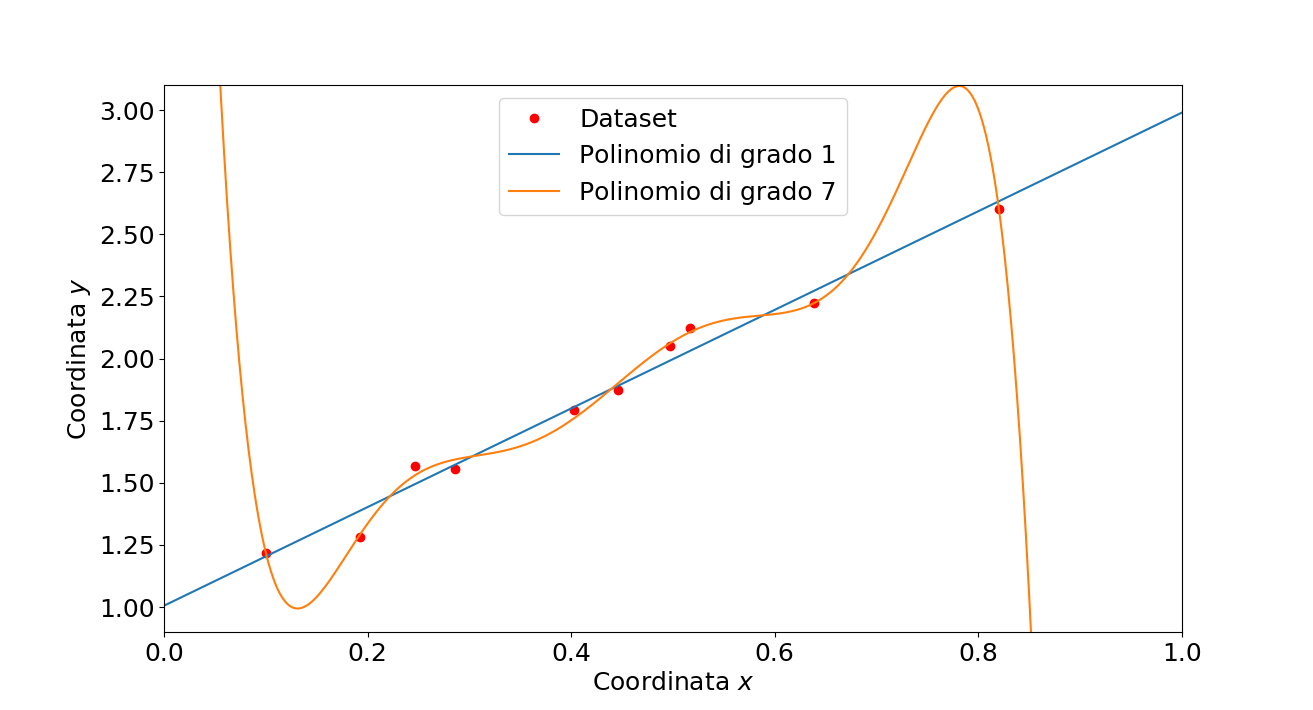
\includegraphics[width=\textwidth]{chapter_1_overfitting_example}
\caption{\textit{In questo esempio, stiamo cercando di trovare un polinomio che meglio approssima i punti del dataset. Il polinomio di grado 7, pur rappresentando esattamente i punti del dataset non ha capacità di generalizzazione, quindi nella pratica si tenderà ad utilizzare il polinomio di grado 1.}}
\label{fig:ch_1_overfitting}
\end{figure}

Questa tecnica è detta \textit{regolarizzazione} (o \textit{regularization}) ed implica l'aggiunta di un \textit{termine di 
regolarizzazione} $R(\bm{\beta})$ alla \textit{loss function}. Nel caso dei regressori lineari il \textit{termine di 
regolarizzazione} imporrà una penalità sul vettore dei pesi che deve essere stimato.
\begin{equation}
\min_{\bm{\beta}} \sum_{i=1}^{n} (\bm{x}_i\bm{\beta} - y_i)^2 - \lambda R(\bm{\beta})
\end{equation}
Il termine $\lambda$ controlla l'importanza della regolarizzazione.
\bigskip

La tecnica utilizzata in entrambi i modelli utilizzati in questo lavoro viene chiamata $\textit{LASSO}$, acronimo per 
\textit{Least Absolute Shrinkage and Selection Operator}. Essa serve a ridurre l'\textit{overfitting} e ad applicare 
una selezione sulle varie feature disponibili. Infatti, un modello regolarizzato con LASSO tenderà ad assegnare un peso 
positivo a poche feature, determinando così quali sono i regressori che contribuiscono in modo maggiore. Inoltre, la 
regolarizzazione LASSO è indicati nei casi di multicollinerità, cioè quando due o più feature sono altamente correlate tra di 
loro (LASSO ne sceglie solo una ed evita di includere nel modello finale le altre, visto che non diminuerebbero l'entropia 
del modello). Nel caso di \textit{LASSO}, il \textit{termine di regolarizzazione} corrisponde alla norma 1, cioè 
$R(\bm{\beta}) = \norm{\bf{\beta}}_1 = \sum_{i=0}^k \beta_i$. 
In questo caso, le due \textit{loss function} \eqref{eq:GLM_minimize} e 
\eqref{eq:GLM_minimize} vengono ridefinite come:
\begin{gather}
\min_{\bm{\beta}} \sum_{i=1}^{n} (\bm{x}_i\bm{\beta} - y_i)^2 + \lambda\norm{\bm{\beta}}_1 \label{eq:OLS_LASSO} \\
\min_{\bm{\beta}} -\sum_{i=1}^n (y_i\theta x_i - e^{\theta x_i} )  + \lambda\norm{\bm{\beta}}_1 \label{eq:GLM_LASSO}
\end{gather}  

Per stimare il parametro $\lambda$ abbiamo utilizzato la tecnica di \textit{cross-validation}. Essa consiste nel suddividere il 
dataset in $k$ partizioni di uguale numerosità, $k-1$ verrano utilizzate per il \textit{training} mentre l'unica rimanente 
verrà utilizzata per il \textit{testing}. La procedura viene poi ripetuta $k$ volte in modo che ogni partizione abbia sia 
stata utilizzata come \textit{testing set}. Attraverso l'utilizzo di questo metodo possiamo avere maggiori informazioni su 
come il modello finale si comporterà con dati nuovi (cioè quanto il modello è capace di generalizzare). Inoltre, questo 
metodo permette appunto di stimare certi parametri del modello, in modo che il loro valore massimizzi le performance 
dell'algoritmo (o minimizzino al meglio la \textit{loss function}).   

\section{Implementazione}

Per la realizzazione del codice, sono stati utilizzati due framework in Python che possiedono l'implementazione dei metodi
sopracitati. La suite \textit{scikit-learn} ha fornito il modello lineare semplice, regolarizzato con \textit{LASSO} e 
validato attraverso \textit{cross-validation}, chiamato \textit{LassoCV}. Per il modello lineare generalizzato di Poisson
è stato usato il framework \textit{glmnet} che ha fornito il metodo \textit{cvglmnet} (anch'esso con \textit{LASSO}+\textit{cross-validation}). 
\bigskip

Entrambe le librerie utilizzate minimizzano funzioni che sono leggermente diverse da quelle presentate precedentemente (in 
particolare \eqref{eq:OLS_LASSO} e \eqref{eq:GLM_LASSO}), che però sono essenzialmente equivalenti ai fini dell'esperimento 
vero e proprio. 
\begin{gather}
	\min_{\bm{\beta}} \frac{1}{2n}\sum_{i=1}^n \norm{\bm{\beta} x_i -y_i}_{2}^2 + \lambda\norm{\bm{\beta}}_1 	\\
	\min_{\bm{\beta}} -\frac{1}{n}\sum_{i=1}^n (y_i\bm{\beta} x_i - e^{\bm{\beta} x_i} ) + \lambda\norm{\bm{\beta}}_1
\end{gather}

\newpage
      \newcommand{\norm}[1]{\left\lVert#1\right\rVert} % norm

\chapter{Metodi}
\bigskip
I metodi che sono stati selezionati per creare i modelli utilizzati negli esperimenti di questo lavoro sono compresi nella 
categoria che in machine learning viene chiamata \textit{apprendimento supervisionato}. Gli algoritmi appartenenti a questo 
gruppo cercano di produrre una funzione $f_a$ che approssimi nel modo migliore un'altra funzione $f_b$ ignota, sulla base di
una serie di dati di esempio (o \textit{osservazioni}) forniti. Attraverso l'utilizzo di questi dati di esempio, si suppone
che l'algoritmo riesca ad accumulare abbastanza ``esperienza" in modo da fornire un'approssimazione della funzione $f_b$. 
\bigskip

Dati $n$ esempi di \textit{training} (che corrispondono al nostro \textit{dataset}), nella forma $\{(y_1, \bm{x}_1), \ldots, (y_n, \bm{x}_n)\}$ dove $y_i$ è il valore associato all'$i$-esimo vettore di \textit{feature} $\bm{x}_i$, l'algoritmo cerca di 
dedurre dalle osservazioni fornite una funzione $f: X \rightarrow Y$, dove $X$ è lo spazio delle \textit{feature} e $Y$ è lo 
spazio del risultato (tale per cui $\forall \; y \in Y$). Questa funzione deve avere anche capacità di generalizzazione, cioè 
deve essere in grado di fare delle previsioni corrette utilizzando come input delle osservazioni che non erano presenti nel 
dataset di training.

\section{Regressione Lineare}
\bigskip

Prevedere i livelli di ILI in Italia, durante la stagione influenzale, a partire dall'analisi delle voci di Wikipedia si 
configura come un problema che viene detto di \textit{regressione}. Con questo termine si indica 
un'ampia classe di problemi il cui obbiettivo è la modellazione di una relazione lineare tra una variabile dipendente $y$ e 
una serie di variabili indipendenti ${x_1, x_2, \ldots, x_n}$ (chiamate anche \textit{regressori}). Nel nostro caso, poichè 
dobbiamo predire una sola variabile dipendente $y$ scalare si parla di \textit{regressione lineare semplice}. 
\bigskip

Più formalmente, dato un dataset $\{ y_i, x_{i1}, x_{i2},\ldots, x_{in}\}^n_i$, la regressione lineare assume che la 
relazione che intercorre tra la variabile dipendente $y_i$ e la variabili indipendenti ${x_{i1}, x_{i2},\ldots, x_{in}}$ sia 
lineare. La relazione viene modellata anche attraverso un variabile aleatoria $\epsilon$ per tenere conto di potenziale 
rumore presente nella dipendenza tra la variabile indipendente e i regressori. Il modello si presenta alla fine come:
\begin{equation}
y_i = \sum_{j=0}^k x_j \cdot \beta_j + \epsilon = \bm{x\cdot\beta}+\epsilon \qquad i=0,1,2,\ldots ,n
\end{equation}

Utilizzando il dataset di \textit{training} si deve "allenare" il modello in modo da stimare correttamente il valore del 
vettore dei pesi $\bm{\beta}$. La tecnica più semplice e anche più frequentemente utilizzata è il \textit{metodo dei minimi 
quadrati} (\textit{ordinary least square})\cite{dismuke2006ordinary}. Esso consiste nell'assegnare ai vari $\beta_i$ dei 
valori che minimizzino una \textit{loss function}, rappresentata dalla somma degli scarti quadratici:
\begin{equation}
\min_{\bm{\beta}} \sum_{i=0}^n(y_i - \bm{x}_i\bm{\beta})^2
\label{eq:OLS_residual}
\end{equation}

Per ottenere ciò, è sufficiente porre tutte le derivate parziali rispetto ad $\beta_i$
uguali a zero, in modo così da trovare il minimo della funzione. Risolvendo le equazioni è possibile arrivare ad ottenere una \textit{closed-form solution} per $\bm{\beta}$ 
(cioè di una espressione matematica che può essere risolta in un numero finito di operazioni). Partendo dall'equazione 
\eqref{eq:OLS_residual}, rappresentata nei passaggi successivi dopo l'espansione del prodotto scalare $\bm{x}_i\bm{\beta}$, 
la dimostrazione è la seguente:
\begin{gather}
	\sum_{i=0}^n\left(\sum_{j=0}^m\left(x_{ij}\beta_j\right)-y_i\right)^2 = 0 \qquad  \\
	\frac{\partial}{\partial\beta_k}\sum_{i=0}^n\left(\sum_{j=0}^m\left(x_{ij}\beta_j\right)-y_i\right)^2 = 0	\qquad \forall \; k=0,\ldots,n \label{eq:OLS_minimize} \\
	\sum_{i=0}^n\frac{\partial}{\partial\beta_k}\left(\sum_{j=0}^m\left(x_{ij}\beta_j\right)-y_i\right)^2 = 0\\
	\sum_{i=0}^n 2\cdot \left(\sum_{j=0}^m \left(x_{ij}\beta_j\right)-y_i\right)\cdot x_{ik} = 0 \\
	\sum_{i=0}^n \bm{x}_{ik}\left(\bm{x}\bm{\beta}-y_i\right) =0 \label{eq:OLS_final}
\end{gather}
Per facilitare le operazioni, si converte la formula \eqref{eq:OLS_final} in notazione matriciale:
\begin{gather}
	X^T \cdot \left( X \bm{\beta} - \bm{y} \right) = 0 \\
	X^T X \bm{\beta} = X^T \bm{y}\\
	\bm{\beta} = \left( X^TX\right)^{-1}X^T\bm{y}
\end{gather}	

Ovviamente esistono altri metodi per stimare il vettore dei pesi $\bm{\beta}$, che variano per complessità 
computazionale dei loro algoritmi, prerequisiti teorici e per la presenza o meno di una \textit{closed-form solution}.  
Il modello di questo progetto utilizza come stimatore l'algoritmo chiamato \textit{coordinate descent}, che permette di trovare minimo locale di una funzione in maniera iterativa.
\bigskip

\section{Modelli Lineari Generalizzati}
\bigskip

Un altro regressore utilizzato in alcuni lavori \cite{McIver2014} per modellare la relazione tra le voci di Wikipedia e l'incidenza di ILI consiste 
in un \textit{modello lineare generalizzato}\cite{GLM} (o \textit{generalized linear model}). Questi modelli assumono che la variabile 
dipendente $y$ non segua una distribuzione normale, ma che possa essere distribuita come una qualsiasi variabile casuale 
della famiglia esponenziale (binomiale, poissoniana, gamma etc.). In questo lavoro di tesi verrà utilizzato un 
\textit{modello lineare generalizzato di Poisson}. 
\bigskip
 
Un modello lineare generalizzato ha bisogno di tre componenti per essere definito correttamente:
\begin{enumerate}
\item Una funzione di distribuzione $f$ facente parte della famiglia esponenziale (in questo caso la funzione di densità di Poisson $p_{\theta}(x) = \frac{\theta^{x}}{x!}e^{-\theta}$);
\item Un predittore lineare $\eta = \bm{x\beta}$, che tenga conto di tutte le variabili indipendenti $\bm{x}_i$;
\item Una funzione invertibile $g$ detta \textit{link function} (normalmente per Poisson viene utilizzato il logaritmo naturale). Questa funzione serve a trasformare il valore atteso della distribuzione $\mathbb{E}(y)$ nel predittore lineare $\eta$, cioè $g(\mathbb{E}(Y)) = \eta$ \label{itm:GML_def_3}.
\end{enumerate}

Di seguito si riporta la procedura per stimare correttamente il vettore dei pesi $\bm{\beta}$ del regressore lineare $\eta$. 
Dato un dataset con $n$ vettori di feature $\bm{x}_i$, un insieme di variabili dipendenti 
associate $y_i$, la probabilità di ottenere la sequenza di valori $y_i$, dati i valori del dataset $\bm{x}_i$ e dato il vettore di pesi $\bm{\beta}$ è:
\begin{equation}
p(y_1,\ldots,y_n | \bm{x}_1,\ldots,\bm{x}_n; \; \bm{\beta}) = \prod_{i=1}^n \frac{e^{\bm{\beta}\bm{x}_iy_i}}{y_i!}e^{-\bm{\beta}\bm{x}_i} \label{eq:GLM_Poisson}
\end{equation}
Questo si può dedurre dalla funzione di densità della distribuzione di Poisson, con il parametro $\theta$ uguale a $e^{\bm{\beta}x_i}$. Si può facilmente dimostrare che $\theta=e^{\bm{\beta}x}$ utilizzando le definizioni precedenti dei modelli lineari generalizzati. Si può infatti notare che il valore atteso per una distribuzione di Poisson e proprio il parametro $\theta$, quindi, per la definizione \ref{itm:GML_def_3}, $\mathbb{E}(y) = \theta = g^{-1}(\eta)$.
\bigskip

Per stimare correttamente il vettore dei pesi viene utilizzata la tecnica della \textit{maximum likelihood 
estimation}, che implica di identificare $\bm{\beta}$ in modo che la probabilità espressa da \eqref{eq:GLM_Poisson} sia
massima. Prima di tutto, si riscrive \eqref{eq:GLM_Poisson} come una \textit{funzione di verosimiglianza}, $\mathcal{L}(\theta | X, Y)$, cioè:
\begin{equation}
\mathcal{L}(\theta | X, Y) = p_{\theta}(x) = p_{\theta}(X=x)
\end{equation}
Quindi, nel caso di una variabile aleatoria di Poisson, la funzione di verosimiglianza diventa:
\begin{equation}
\mathcal{L}(\bm{\beta x}  | X, Y ) = \prod_{i=1}^n {e^{y_i \bm{\beta} x_i}-e^{-\bm{\beta} x_i}}{y_i!} \label{eq:GLM_Likelihood}
\end{equation}
Per semplificare i calcoli, spesso si utilizza una versione semplificata della funzione di verosimiglianza, la \textit{log-likelihood function}, $l(\theta | X, Y)$ che corrisponde ad applicare il logaritmo naturale a \eqref{eq:GLM_Likelihood}, cioè 
$l(\bm{\beta x}  | X, Y) = \log{\mathcal{L}(\bm{\beta x}  | X, Y )}$. 
Eseguendo le dovute semplificazioni, la funzione di verosimiglianza da minimizzare (attraverso tecniche di \textit{gradient descent}) diventa quindi:
\begin{equation}
	\min_{\bm{\beta}} -\sum_{i=1}^n (y_i\bm{\beta} x_i - e^{\bm{\beta} x_i} ) \label{eq:GLM_minimize}
\end{equation} 

\section{Regolarizzazione}
\bigskip

Come si è precedentemente detto, utilizzando vari stimatori (\textit{coordinate descent} e \textit{maximum likelihood}) 
si stimano i valori dei pesi che andranno poi a formare il nostro regressore lineare. Nonostante tutto, questi metodi 
non sono privi di errori e possono incappare in problemi cosiddetti di \textit{overfitting}, causati principalmente da un 
numero eccessivo di parametri rispetto al totale delle osservazioni. In questi casi, il modello potrebbe descrivere 
perfettamente i dati del dataset di training, ma non essere comunque abbastanza generale da fornire previsioni corrette con 
ulteriori dati di test (si veda l'esempio mostrato in Figura \ref{fig:ch_1_overfitting}). 
Pertanto, all'interno delle funzioni da minimizzare precedentemente citate, in particolare \eqref{eq:OLS_minimize} e 
\eqref{eq:GLM_minimize}, abbiamo inserito una penalità che ci permetterà di ottenere un modello meno sensibile 
all'\textit{overfitting}. 
\bigskip 

\begin{figure}[!ht]
\centering
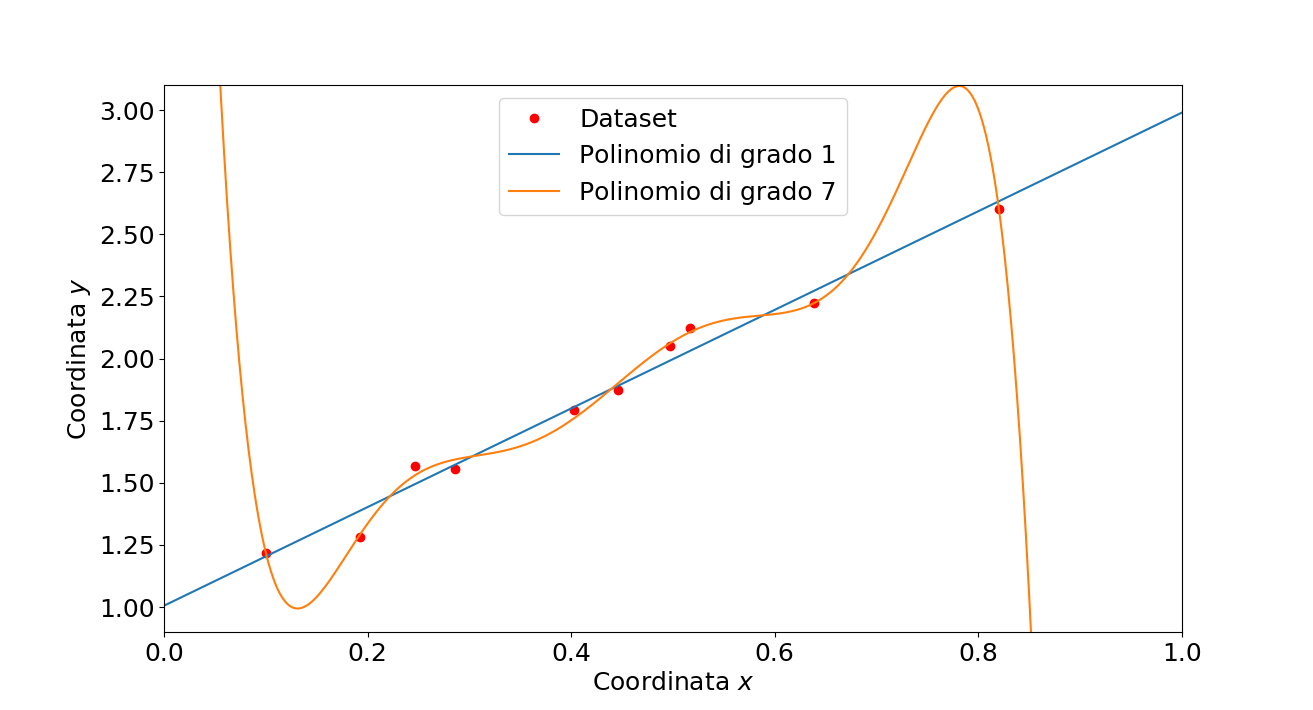
\includegraphics[scale=0.5]{chapter_1_overfitting_example}
\caption{\textit{In questo esempio, stiamo cercando di trovare un polinomio che meglio approssima i punti del dataset. Il polinomio di grado 7, pur rappresentando esattamente i punti del dataset non ha capacità di generalizzazione, quindi nella pratica si tenderà ad utilizzare il polinomio di grado 1.}}
\label{fig:ch_1_overfitting}
\end{figure}

Questa tecnica è detta \textit{regolarizzazione} (o \textit{regularization}) e implica l'aggiunta di un \textit{termine di 
regolarizzazione} $R(\bm{\beta})$ alla \textit{loss function}. Nel caso dei regressori lineari il \textit{termine di 
regolarizzazione} imporrà una penalità sul vettore dei pesi che deve essere stimato.
\begin{equation}
\min_{\bm{\beta}} \sum_{i=1}^{n} (y_i - \bm{x}_i\bm{\beta})^2 - \lambda R(\bm{\beta})
\end{equation}
Il termine $\lambda$ controlla l'importanza della regolarizzazione.
\bigskip

La tecnica utilizzata in entrambi i modelli proposti in questo lavoro viene chiamata $\textit{LASSO}$, acronimo per 
\textit{Least Absolute Shrinkage and Selection Operator}. Essa serve a ridurre l'\textit{overfitting} e ad applicare 
una selezione sulle varie feature disponibili. Infatti, un modello regolarizzato con LASSO tenderà ad assegnare un peso 
diverso da zero a poche feature, privilegiando i regressori che contribuiscono in modo maggiore. Inoltre, la 
regolarizzazione LASSO è indicata nei casi di multicollinerità, cioè quando due o più feature sono altamente correlate tra di 
loro (LASSO ne sceglie solo una ed evita di includere nel modello finale le altre, visto che non diminuirebbero l'entropia 
del modello). Nel caso di \textit{LASSO}, il \textit{termine di regolarizzazione} corrisponde alla norma 1, cioè 
$R(\bm{\beta}) = \norm{\bf{\beta}}_1 = \sum_{i=0}^k \beta_i$. 
In questo caso, le due \textit{loss function} \eqref{eq:GLM_minimize} e 
\eqref{eq:GLM_minimize} vengono ridefinite come:
\begin{gather}
\min_{\bm{\beta}} \sum_{i=1}^{n} (\bm{x}_i\bm{\beta} - y_i)^2 + \lambda\norm{\bm{\beta}}_1 \label{eq:OLS_LASSO} \\
\min_{\bm{\beta}} -\sum_{i=1}^n (y_i\theta x_i - e^{\theta x_i} )  + \lambda\norm{\bm{\beta}}_1 \label{eq:GLM_LASSO}
\end{gather}  

Per stimare il parametro $\lambda$ si è utilizzata la tecnica di \textit{cross-validation}. Essa consiste nel suddividere il 
dataset in $k$ partizioni disgiunte di uguale numerosità, $k-1$ verrano utilizzate per il \textit{training} mentre l'unica 
rimanente verrà utilizzata per il \textit{testing}. La procedura viene poi ripetuta $k$ volte in modo che ogni partizione 
sia stata utilizzata come \textit{testing set}. Attraverso l'utilizzo di questo metodo possiamo avere maggiori 
informazioni su come il modello finale si comporterà con nuovi dati (cioè quanto il modello sarà in grado di generalizzare). 
Inoltre, questo metodo permette appunto di stimare certi parametri del modello, in modo che il loro valore massimizzi le 
performance dell'algoritmo (o minimizzino al meglio la \textit{loss function}).   

\section{Implementazione}
\bigskip

Per la realizzazione del codice, sono stati utilizzati due framework in Python che possiedono l'implementazione dei metodi
sopracitati. La suite \textit{scikit-learn} \cite{scikit-learn} ha fornito il modello lineare semplice, regolarizzato con 
\textit{LASSO} e validato attraverso \textit{cross-validation}, chiamato \textit{LassoCV}. Per il modello lineare 
generalizzato di Poisson è stato usato il framework \textit{glmnet} \cite{GLMNET} che ha fornito il metodo \textit{cvglmnet} 
(anch'esso con \textit{LASSO}+\textit{cross-validation}). Entrambe le librerie minimizzano funzioni che sono 
leggermente diverse da quelle presentate precedentemente (in particolare \eqref{eq:OLS_LASSO} e \eqref{eq:GLM_LASSO}), che 
però sono essenzialmente equivalenti ai fini dell'esperimento vero e proprio. 
\begin{gather}
	\min_{\bm{\beta}} \frac{1}{2n}\sum_{i=1}^n \norm{\bm{\beta} x_i -y_i}_{2}^2 + \lambda\norm{\bm{\beta}}_1 	\qquad
	\min_{\bm{\beta}} -\frac{1}{n}\sum_{i=1}^n (y_i\bm{\beta} x_i - e^{\bm{\beta} x_i} ) + \lambda\norm{\bm{\beta}}_1
\end{gather}

\newpage
      \chapter{Risultati}
\bigskip

\section{Risultati del modello lineare}
\bigskip

Per valutare le performance del modello lineare, oltre ai sistemi classici come l'\textit{errore quadratico medio}, abbiamo 
cercato di misurare con che precisione il modello tende a predire il picco influenzale, cioè la settimana con la massima 
incidenza della patologia nella popolazione italiana. Come si può notare dalla Tabella \ref{tab:models_results}, nella metà 
delle stagioni influenzali il modello lineare predice il picco entro una settimana indicata dai dati InfluNet; inoltre, nelle 
stagioni 2008-2009, 2011-2012 e 2014-2015 il picco è previsto correttamente. Negli altri quattro casi il modello lineare 
tende ad anticipare la settimana del picco (stagioni 2007-2008, 2010-2011 e 2013-2014).
\bigskip

Il modello lineare possiede una buona capacità predittiva anche nel caso della stagione influenzale 2009-2010, che fu 
particolarmente grave poiché ci fu una vera e propria epidemia causata dalla varietà H1N1 del virus influenzale. Il picco in 
questo caso è spostato verso le ultime settimane del 2009 (dalla numero 42 alla 52) e non corrisponde all'andamento 
classico della patologia (si nota molto bene dalla Figura \ref{fig:ch_2_ILI_levels}). Inoltre, quell'anno c'era stata una 
grande copertura mediatica riguardo all'epidemia, cosa che avrebbe potuto in qualche modo aggiungere rumore ai dati del 
dataset. Nonostante ciò, il modello riesce a prevedere il picco della stagione correttamente (con uno scarto di una 
settimana).
\bigskip

Abbiamo anche cercato di individuare quali feature siano più importanti per la previsione dei valori di incidenza. Ci siamo 
soffermati su quelle voci di Wikipedia che sono presenti più volte in tutti i modelli e quali di esse avessero il più grande 
peso $\beta_i$ associato. Attraverso l'utilizzo di LASSO abbiamo potuto ridurre considerevolmente il numero di feature che 
effettivamente giocano un ruolo nella previsione dell'incidenza, infatti, da 470 feature, i modelli ne andavano 
ad utilizzare in media 111 (con utilizzare si intende che veniva assegnato loro un peso $\beta_i \neq 0$). 
\bigskip

La Tabella \ref{tab:models_features} mostra le prime 5 feature con peso medio maggiore e in quanti modelli 
esse siano presenti. Come si può notare, sono voci di Wikipedia legate ai sintomi influenzali (la voce con più alto 
peso medio riguarda la patologia \textit{Febbre}). Poiché quasi nel 100\% dei modelli abbiamo le stesse feature, e poiché 
esse danno il contributo più grande nel determinare il livello di incidenza influenzale, possiamo supporre che anche 
l'andamento delle pageview di queste voci rispecchi l'andamento dei dati InfluNet e che quindi pageview ed InfluNet siano in 
qualche modo correlati.
\bigskip

Questa relazione è facilmente visibile ad esempio nella stagione influenzale 2012-2013, come ci mostra la Figura 
\ref{fig:ch_3_correlation_linear}. Se osserviamo l'andamento delle pageview di alcune delle voci della Tabella 
\ref{tab:models_features} rispetto all'incidenza ILI, si può notare come il loro valore inizi ad aumentare esattamente 
nello stesso periodo in cui anche l'incidenza della patologia aumenta. Questa relazione si può osservare anche nelle stagioni 
influenzali 2009-2010 e 2011-2012.
\bigskip

Per verificare che questa relazione tra le pageview e l'incidenza ILI in Italia si presenti solo con pagine legate all'ambito 
medico, in particolare con pagine legate alla patologia influenzale, abbiamo provato ad 
utilizzare il dataset formato da voci estratte casualmente da Wikipedia per allenare il modello lineare, con le stesse 
modalità con cui abbiamo usato quello reale. Come ci aspettavamo, utilizzando le pagine casuali, il modello non riesce ad 
effettuare previsioni coerenti con InfluNet. In certe stagioni influenzali, il modello non riesce neppure a convergere ad una 
soluzione e molto spesso alla quasi totalità delle 470 feature non viene assegnato nessun peso $\beta_i$ diverso da zero. Ciò 
significa che probabilmente non esiste una relazione lineare tra le pageview del dataset casuale e l'incidenza InfluNet, a 
differenza di ciò che accade con il dataset formato da pagine di categoria medica.
\bigskip

\begin{table}[p]
\centering
\begin{adjustbox}{max width=\textwidth}
\begin{tabular}{|c|c|c|c|c|c|}
\hline
\rowcolor[HTML]{EFEFEF} 
\textbf{Stagione Influenzale} & \textbf{Picco IN (Settimana)} & \textbf{Picco M (Settimana)} & \textbf{Picco IN} & \textbf{Picco M} & \textbf{MSE}   \\ \hline
\multicolumn{6}{|c|}{\cellcolor[HTML]{EFEFEF}Modello Lineare} \\ \hline
\textit{2007-2008}            & \textit{5}                          & \textit{1}                    & \textit{7.21}           & \textit{1.64}     & \textit{11.00} \\ \hline
\rowcolor[HTML]{FFFFFF} 
\textit{2008-2009}            & \textit{4}                          & \textit{4}                    & \textit{8.23}           & \textit{6.64}     & \textit{4.43}  \\ \hline
\rowcolor[HTML]{FFFFFF} 
\textit{2009-2010}            & \textit{46}                         & \textit{45}                   & \textit{12.92}          & \textit{10.89}    & \textit{5.02}  \\ \hline
\rowcolor[HTML]{FFFFFF} 
\textit{2010-2011}            & \textit{5}                          & \textit{4}                    & \textit{11.04}          & \textit{14.80}    & \textit{7.35}  \\ \hline
\rowcolor[HTML]{FFFFFF} 
\textit{2011-2012}            & \textit{5}                          & \textit{5}                    & \textit{9.64}           & \textit{7.99}     & \textit{1.29}  \\ \hline
\rowcolor[HTML]{FFFFFF} 
\textit{2012-2013}            & \textit{6}                          & \textit{5}                    & \textit{9.99}           & \textit{11.95}    & \textit{2.67}  \\ \hline
\rowcolor[HTML]{FFFFFF} 
\textit{2013-2014}            & \textit{6}                          & \textit{3}                    & \textit{6.67}           & \textit{13.80}    & \textit{7.38}  \\ \hline
\rowcolor[HTML]{FFFFFF} 
\textit{2014-2015}            & \textit{4}                          & \textit{4}                    & \textit{10.87}          & \textit{5.11}     & \textit{7.18}  \\ \hline
\rowcolor[HTML]{FFFFFF} 
\textit{2015-2016}            & \textit{8}                          & \textit{5}                    & \textit{6.14}           & \textit{5.59}     & \textit{2.55}  \\ \hline
\rowcolor[HTML]{EFEFEF} 
\multicolumn{6}{|c|}{\cellcolor[HTML]{EFEFEF}Modello di Poisson} \\ \hline
\textit{2007-2008}            & \textit{5}                          & \textit{1}                    & \textit{7.21}           & \textit{1.01}     & \textit{13.02}    \\ \hline
\rowcolor[HTML]{FFFFFF} 
\textit{2008-2009}            & \textit{4}                          & \textit{4}                    & \textit{8.23}           & \textit{5.78}     & \textit{3.31}     \\ \hline
\rowcolor[HTML]{FFFFFF} 
\textit{2009-2010}            & \textit{46}                         & \textit{45}                   & \textit{12.92}          & \textit{1090.86}  & \textit{44764.56} \\ \hline
\rowcolor[HTML]{FFFFFF} 
\textit{2010-2011}            & \textit{5}                          & \textit{6}                    & \textit{11.04}          & \textit{59.16}    & \textit{147.97}   \\ \hline
\rowcolor[HTML]{FFFFFF} 
\textit{2011-2012}            & \textit{5}                          & \textit{5}                    & \textit{9.64}           & \textit{8.57}     & \textit{1.27}     \\ \hline
\rowcolor[HTML]{FFFFFF} 
\textit{2012-2013}            & \textit{6}                          & \textit{8}                    & \textit{9.99}           & \textit{8.45}     & \textit{6.25}     \\ \hline
\rowcolor[HTML]{FFFFFF} 
\textit{2013-2014}            & \textit{6}                          & \textit{3}                    & \textit{6.67}           & \textit{16.48}    & \textit{6.15}     \\ \hline
\rowcolor[HTML]{FFFFFF} 
\textit{2014-2015}            & \textit{4}                          & \textit{5}                    & \textit{10.87}          & \textit{4.95}     & \textit{9.73}     \\ \hline
\rowcolor[HTML]{FFFFFF} 
\textit{2015-2016}            & \textit{8}                          & \textit{7}                    & \textit{6.14}           & \textit{5.23}     & \textit{2.64}     \\ \hline
\end{tabular}
\end{adjustbox}
\caption{\textit{Per ogni stagione influenzale e per ogni modello sono stati registrati: la settimana in cui è presente il 
picco massimo di incidenza ILI indicato dai dati InfluNet, la settimana con il picco massimo di incidenza predetto dai 
modelli, il valore dell'incidenza del picco massimo di InfluNet, il valore dell'incidenza del picco massimo predetto dai modelli e l'MSE (Mean Squared Error), per misurare le prestazioni dei modelli nelle varie stagioni influenzali. Con la sigla IN si intende il valore indicato dai dati InfluNet, mentre con M si indica il valore predetto dai modelli.}}
\label{tab:models_results}
\end{table}

\begin{table}[p]
\centering
\begin{adjustbox}{max width=\textwidth}
\begin{tabular}{|l|l|l|}
\hline
\rowcolor[HTML]{EFEFEF} 
\textbf{Feature}                            & \textbf{Peso Medio} & \textbf{Modelli in cui è presente} \\ \hline
\rowcolor[HTML]{EFEFEF} 
\multicolumn{3}{|c|}{\cellcolor[HTML]{EFEFEF}Modello Lineare} \\ \hline
\textit{Febbre}                             & \textit{13.11}      & \textit{9/9}                                            \\ \hline
\textit{Influenza}                          & \textit{4.71}       & \textit{9/9}                                            \\ \hline
\textit{Bronchite}                          & \textit{4.64}       & \textit{9/9}                                            \\ \hline
\textit{Influenzavirus\_A\_sottotipo\_H1N1} & \textit{3.98}       & \textit{8/9}                                            \\ \hline
\textit{Polipnea}                           & \textit{3.01}       & \textit{9/9}                                            \\ \hline
\rowcolor[HTML]{EFEFEF} 
\multicolumn{3}{|c|}{\cellcolor[HTML]{EFEFEF}Modello di Poisson} \\ \hline
\textit{Pagina principale}                      & \textit{0.52}                              & \textit{9/9}                                              \\ \hline
\textit{Febbre ricorrente}                      & \textit{0.07}                              & \textit{9/9}                                              \\ \hline
\textit{Vaccino per la febbre tifoide}          & \textit{0.06}                              & \textit{2/9}                                              \\ \hline
\textit{Stimmate\_(medicina)}                   & \textit{0.05}                              & \textit{8/9}                                              \\ \hline
\textit{Virus dell'encefalite di Murray Valley} & \textit{0.05}                              & \textit{2/9}                                              \\ \hline
\end{tabular}
\end{adjustbox}
\caption{\textit{Tabella indicante le feature utilizzate dai modelli ordinate per il loro peso medio.}}
\label{tab:models_features}
\end{table}

Osservando i grafici successivi (Figura \ref{fig:appendix_linear}), si osserva come il modello lineare sia più efficace 
nelle stagioni influenzali che vanno dalla 2008-2009 fino alla 2012-2014, mentre si comporta relativamente peggio nelle 
stagioni 2007-2008, 2014-2015 e 2015-2016. Le basse prestazioni possono essere spiegati nel seguente modo: 
\begin{itemize}
\item Nel caso della stagione 2007-2008 alcune delle voci utilizzate dal modello non erano ancora ancora presenti come 
pagine di Wikipedia, quindi il valore delle pageview settimanali per la stagione 2007-2008 per queste feature non è 
disponibile. Infatti, su 470 feature, 184 sono "nulle", mentre delle 51 feature utilizzate dal modello 18 di queste hanno 
valori sempre uguali a zero nel dataset che copre l'arco di tempo 2007-2008. Probabilmente, a causa di ciò il modello ha 
stimato valori di incidenza ILI più bassi del normale, poiché non aveva sufficienti informazioni per dare una previsione 
corretta;
\item Nel caso delle stagioni 2014-2015 e 2015-2016, la causa può essere imputata principalmente alla mancanza di una 
variazione significativa dei valori delle pageview per le voci selezionate dal modello. In sostanza, a differenza del 
2012-2013, in cui l'andamento delle voci seguiva quello dell'incidenza ILI, nel 2014-2015 e 2015-2016 ciò non succede. 
Questo potrebbe essere causato dalla mancanza nel dataset di informazioni riguardanti gli accessi tramite dispositivi mobile 
che, se aggiunte, potrebbero migliorare le prestazioni (che come si è detto nel capitolo precedente, ora sono maggioritarie 
rispetto ai semplici accessi via desktop).
\end{itemize}

\begin{figure}[ht]
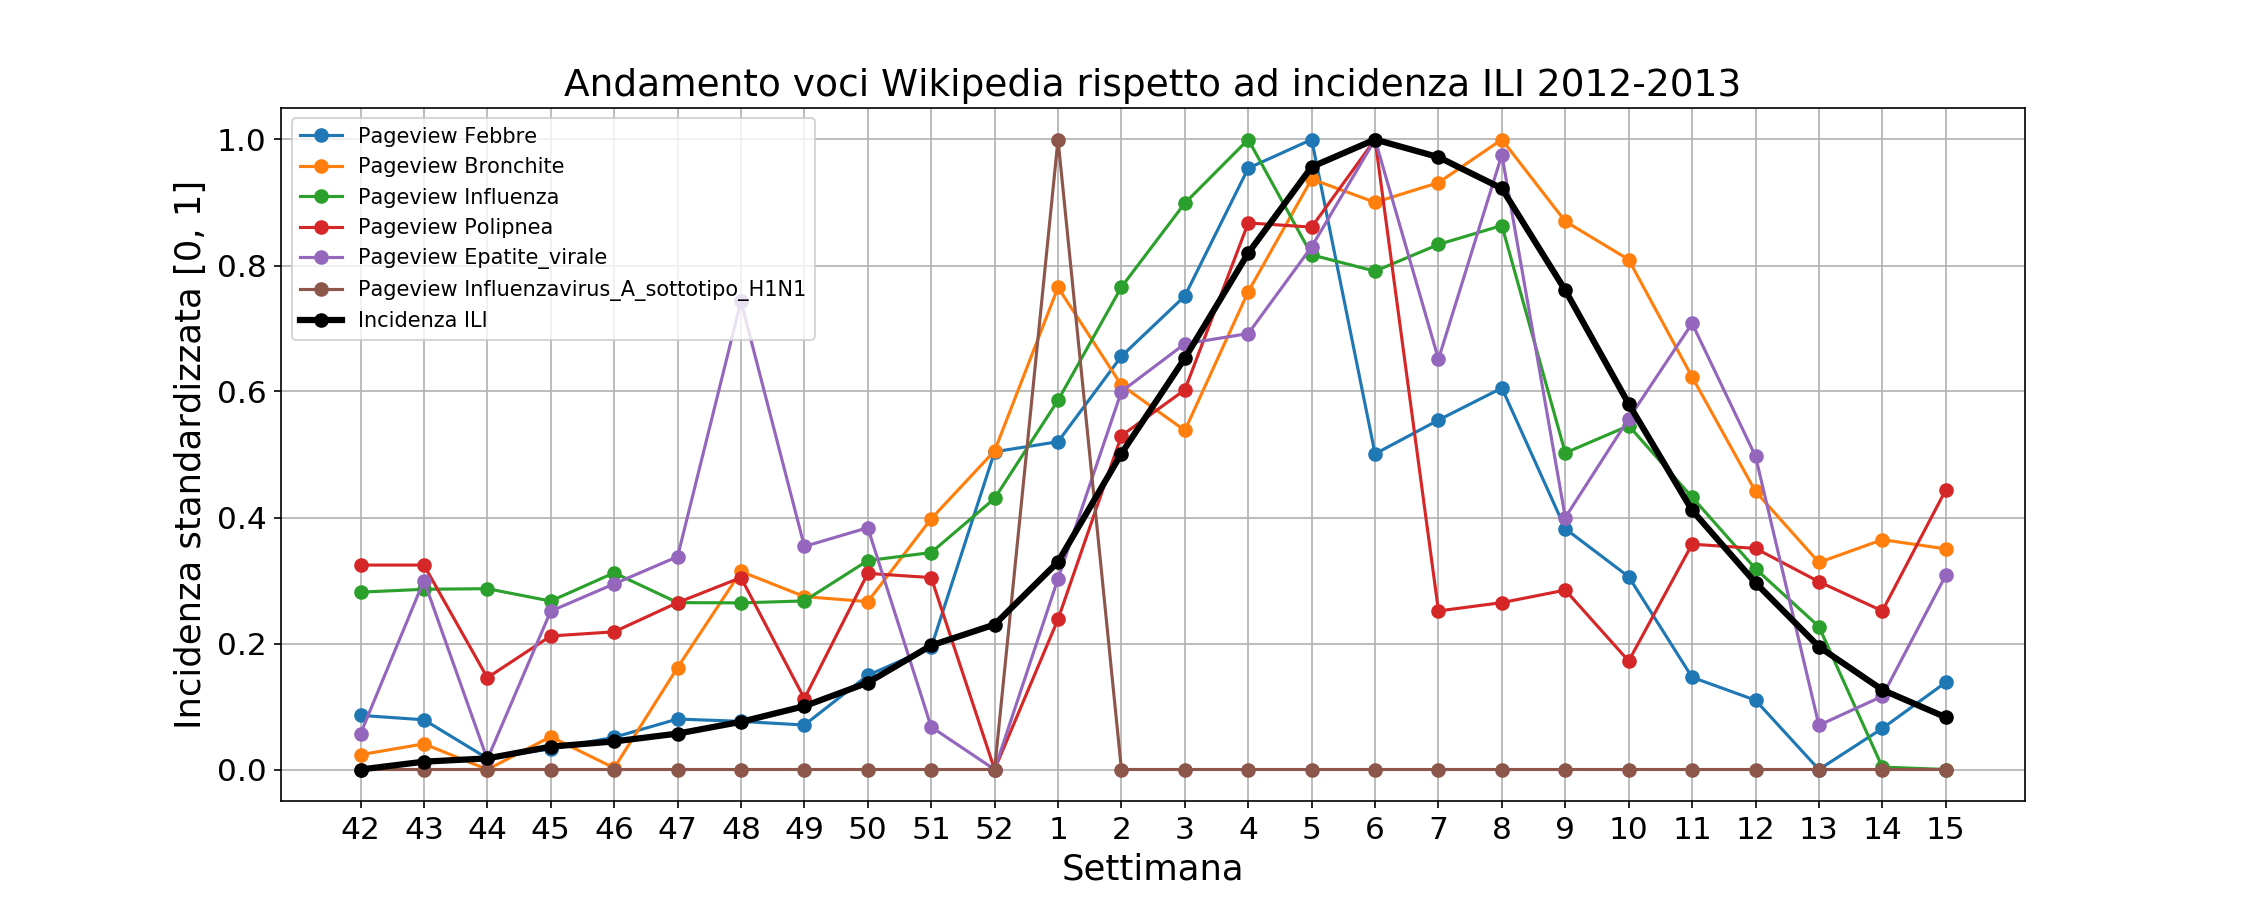
\includegraphics[width=\textwidth]{chapter_3_correlation_linear}
\caption{\textit{Variazione del valore di alcune feature rispetto all'incidenza ILI (i valori per essere comparati sono stati normalizzati nell'intervallo [0,1]).}}
\label{fig:ch_3_correlation_linear}
\centering
\end{figure}

\section{Risultati del modello di Poisson}
\bigskip

Per valutare le prestazioni del modello di Poisson abbiamo proceduto come abbiamo fatto per il modello lineare, osservando 
con quanta efficacia vengono previsti i picchi influenzali, il loro valore e l'andamento generale dell'incidenza ILI. 
Nonostante nel paper di riferimento \cite{McIver2014} l'utilizzo di un modello generalizzato si sia rivelato efficace e 
adatto a stimare i livelli di ILI, per l'Italia il modello di Poisson non ha mostrato significativi miglioramenti rispetto al 
modello lineare, anzi in certi casi ha mostrato un calo di prestazioni. Come mostra la Tabella 
\ref{tab:models_results}, pur riuscendo a stimare il picco influenzale (con uno scarto di una settimana) in cinque 
stagioni su nove, il modello tende in alcuni casi a sovrastimare in maniera abbondante l'incidenza del picco.
\bigskip

Riguardo invece alle feature utilizzate, osservando la Tabella \ref{tab:models_features}, si nota come il modello di 
Poisson tenda a dare maggior peso a voci di Wikipedia che poco hanno a che fare con i sintomi della patologia influenzale. 
Inoltre, i pesi assegnati hanno un entità molto minore rispetto a quelli del modello lineare e  
l'andamento delle feature rispetto al valore dell'incidenza ILI non ha una corrispondenza così netta (Figura 
\ref{fig:ch_3_correlation_poisson}).
\bigskip

Il modello è anche poco resistente agli \textit{outliers} presenti nel dataset di Wikipedia. Infatti, come si nota dai 
grafici in Figura \ref{fig:appendix_poisson}, nella sesta settimana del 2011 e
nella terza e nona settimana del 2014, il modello stima dei valori di incidenza ILI molto elevati, rispetto a quanto indicato 
dai dati Influnet. Questi sono per lo più causati da voci di Wikipedia che in quelle specifiche settimane hanno ricevuto un 
totale di visite che si discosta in maniera evidente dalla loro media settimanale (probabilmente a causa di alcuni bot).
\bigskip 

Per confermare comunque che questi risultati si ottengono soltanto quando si analizzano le voci di categoria medica di 
Wikipedia, abbiamo provato ad utilizzare il dataset composto da voci casuali e l'esito è stato lo stesso di quello ottenuto 
con il modello lineare. Il modello generalizzato non riesce a prevedere con sufficiente accuratezza ne i picchi influenzali, 
ne il normale andamento dell'incidenza ILI. 
\bigskip

Il modello di Poisson ha lo stesso comportamento del modello lineare per quanto riguarda le stagioni influenzali 2007-2008, 
2014-2015 e 2015-2016. Le basse prestazioni in quei casi possono essere addotte alle stesse motivazioni presentate per il 
modello lineare, cioè la mancanza di una parte significativa delle \textit{page view} dal dataset e con un numero troppo 
elevato di predittori nulli.
\bigskip

Un altra motivo per cui le prestazioni non sono ottimali potrebbero essere il fatto che la regressione di Poisson assume 
che la variabile aleatoria dipendente (cioè in questo caso il valore di incidenza ILI) segua la distribuzione di Poisson. 
Questo porta con se una condizione abbastanza restrittiva che implica che la sua media e la sua varianza devono essere 
uguali, cosa che non è sempre vera nei dataset reali. Infatti, si può notare come in tutte le stagioni influenzali 
l'incidenza ILI tenda a seguire una distribuzione normale (che quindi è più adatta ad essere prevista con un semplice modello 
lineare) rendendo quindi difficile l'utilizzo di questo metodo per costruire un modello predittivo.
\bigskip

\begin{figure}[h]
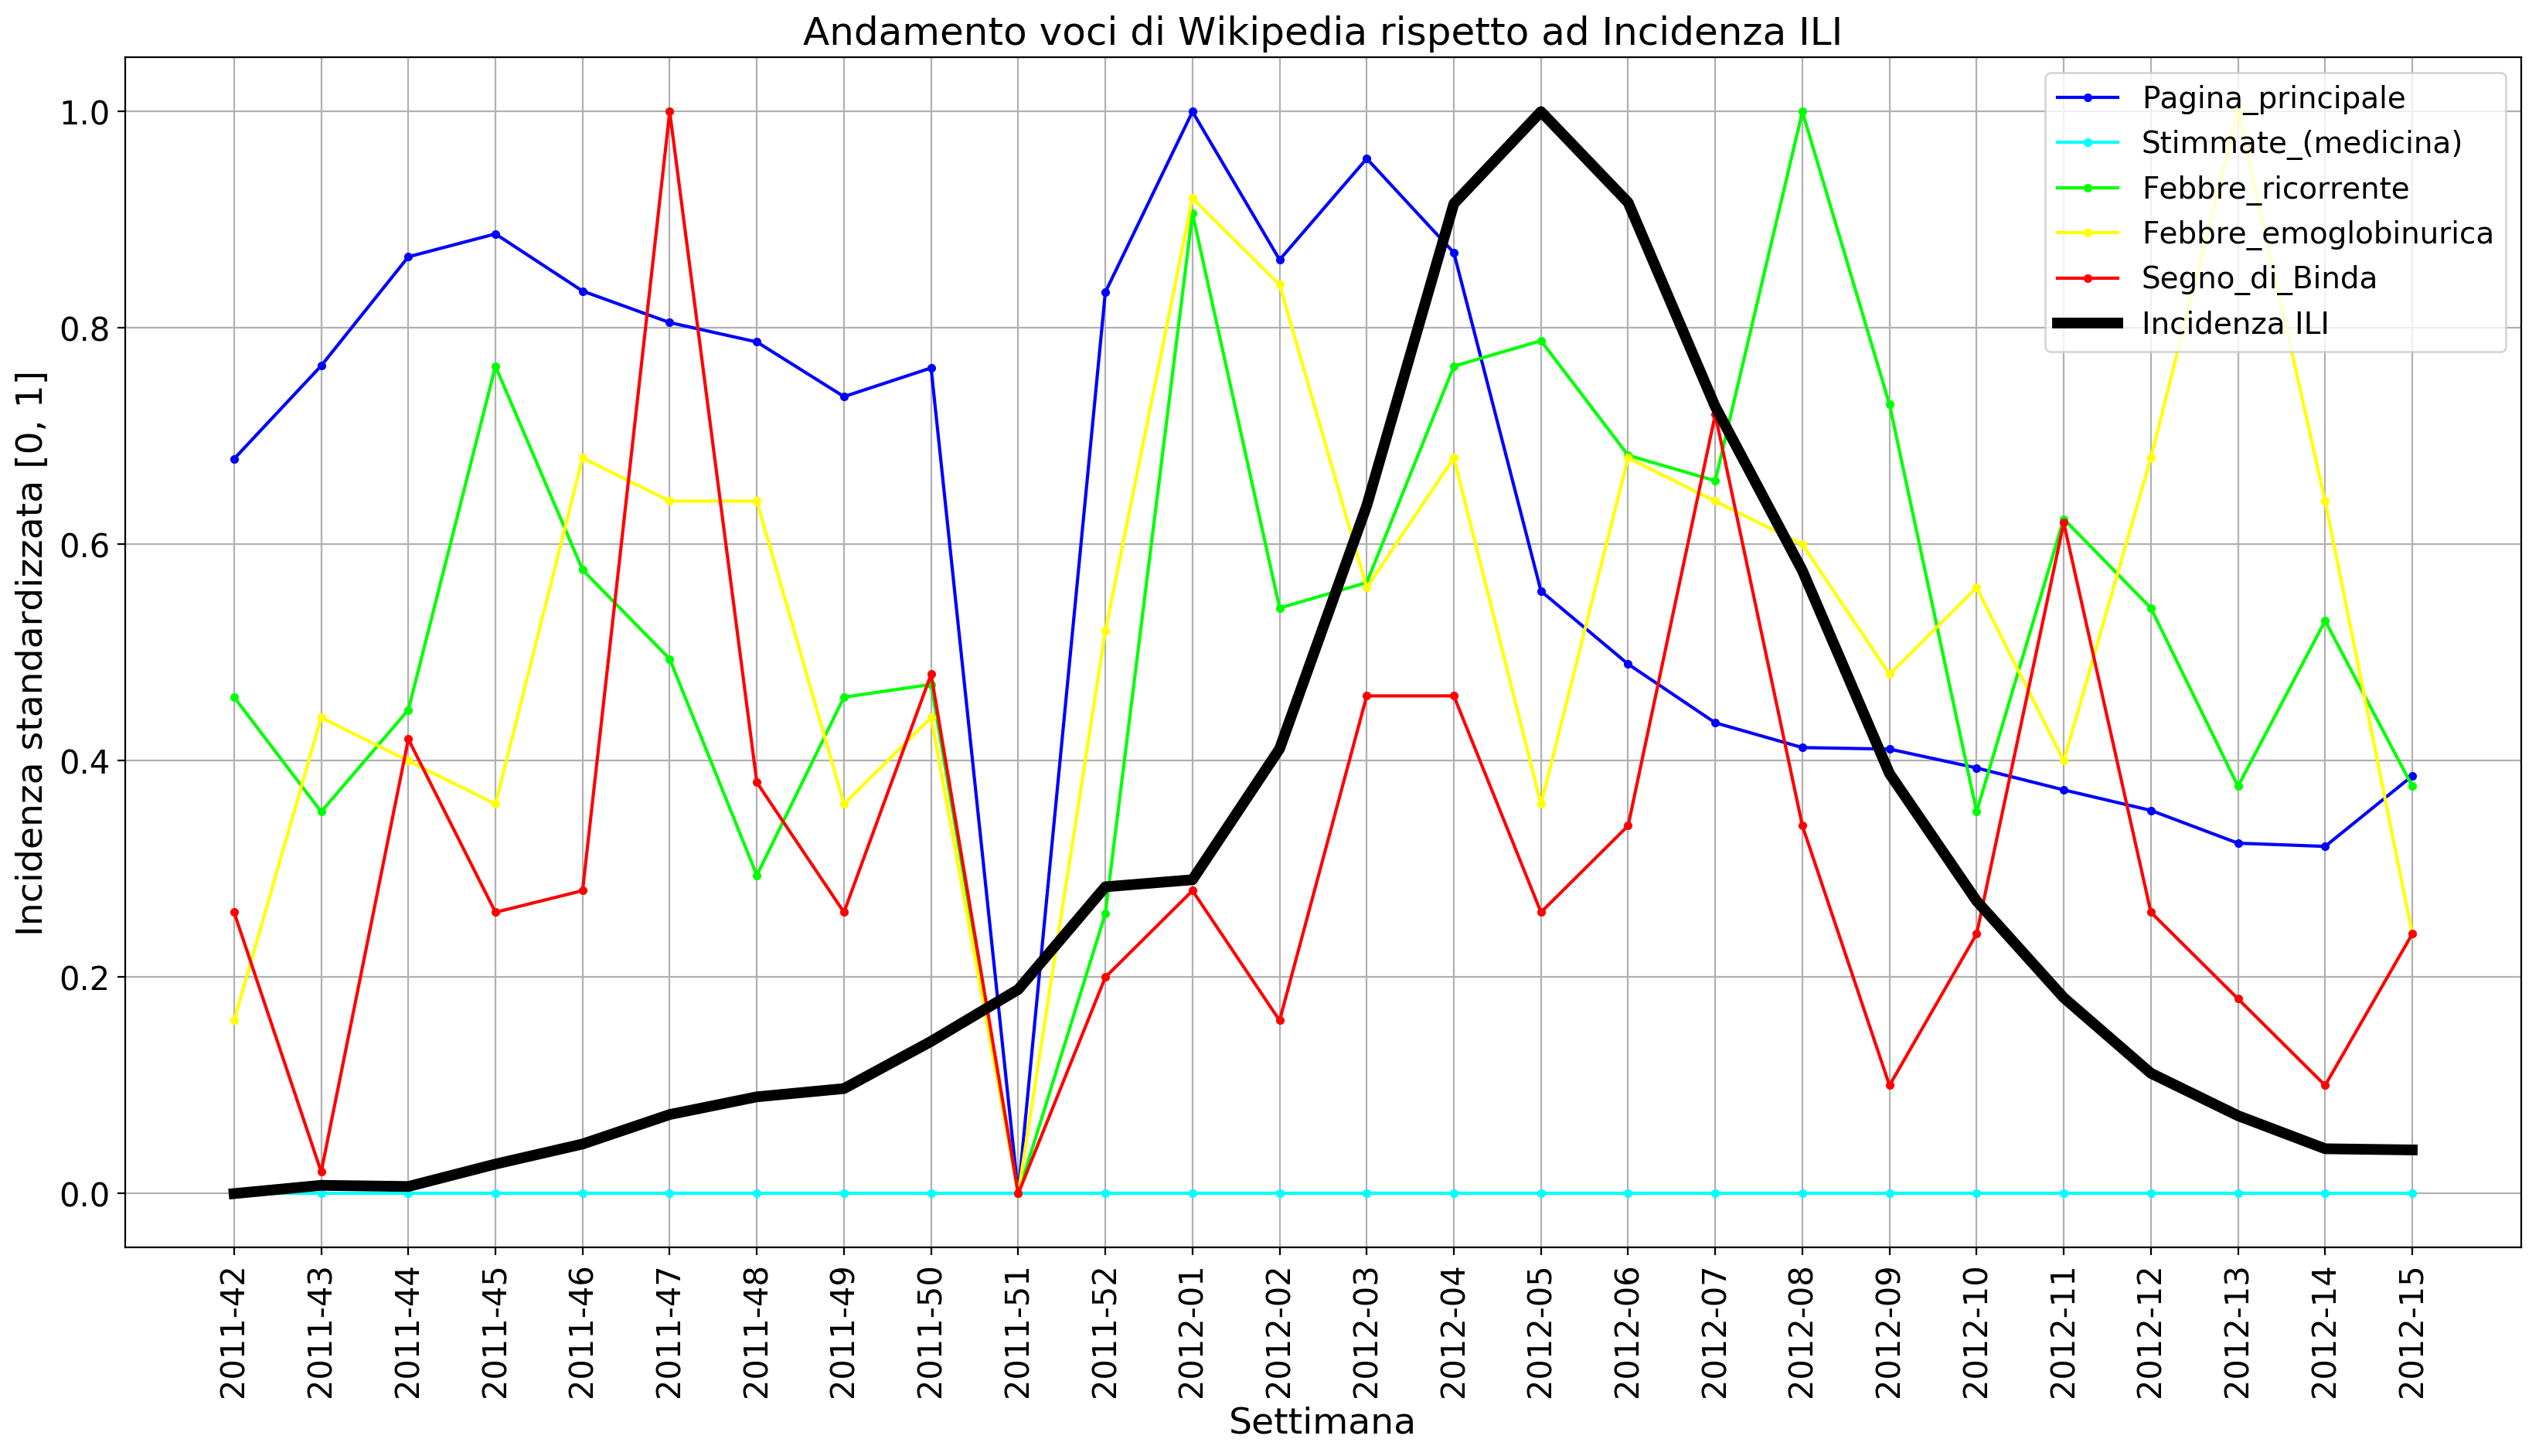
\includegraphics[width=\textwidth]{chapter_3_correlation_poisson}
\caption{\textit{Variazione del valore delle prime 5 feature rispetto all'incidenza ILI (i valori per essere comparati sono stati normalizzati nell'intervallo [0,1]).}}
\label{fig:ch_3_correlation_poisson}
\centering
\end{figure}

\clearpage
      %\input{capitolo4}
      
      
    \endgroup


    % bibliografia in formato bibtex
    %
    % aggiunta del capitolo nell'indice
    \addcontentsline{toc}{chapter}{Bibliografia}
    % stile con ordinamento alfabetico in funzione degli autori
    \bibliographystyle{unsrt}
    \bibliography{biblio}
%%%%%%%%%%%%%%%%%%%%%%%%%%%%%%%%%%%%%%%%%%%%%%%%%%%%%%%%%%%%%%%%%%%%%%%%%%
%%%%%%%%%%%%%%%%%%%%%%%%%%%%%%%%%%%%%%%%%%%%%%%%%%%%%%%%%%%%%%%%%%%%%%%%%%
%% Nota
%%%%%%%%%%%%%%%%%%%%%%%%%%%%%%%%%%%%%%%%%%%%%%%%%%%%%%%%%%%%%%%%%%%%%%%%%%
%% Nella bibliografia devono essere riportati tutte le fonti consultate 
%% per lo svolgimento della tesi. La bibliografia deve essere redatta 
%% in ordine alfabetico sul cognome del primo autore. 
%% 
%% La forma della citazione bibliografica va inserita secondo la fonte utilizzata:
%% 
%% LIBRI
%% Cognome e iniziale del nome autore/autori, la data di edizione, titolo, casa editrice, eventuale numero dell’edizione. 
%% 
%% ARTICOLI DI RIVISTA
%% Cognome e iniziale del nome autore/autori, titolo articolo, titolo rivista, volume, numero, numero di pagine.
%% 
%% ARTICOLI DI CONFERENZA
%% Cognome e iniziale del nome autore/autori (anno), titolo articolo, titolo conferenza, luogo della conferenza (città e paese), date della conferenza, numero di pagine. 
%% 
%% SITOGRAFIA
%% La sitografia contiene un elenco di indirizzi Web consultati e disposti in ordine alfabetico. 
%% E’ necessario:
%%   Copiare la URL (l’indirizzo web) specifica della pagina consultata
%%   Se disponibile, indicare il cognome e nome dell’autore, il titolo ed eventuale sottotitolo del testo
%%   Se disponibile, inserire la data di ultima consultazione della risorsa (gg/mm/aaaa).    
%%%%%%%%%%%%%%%%%%%%%%%%%%%%%%%%%%%%%%%%%%%%%%%%%%%%%%%%%%%%%%%%%%%%%%%%%%
%%%%%%%%%%%%%%%%%%%%%%%%%%%%%%%%%%%%%%%%%%%%%%%%%%%%%%%%%%%%%%%%%%%%%%%%%%
    

    \titleformat{\chapter}
       {\normalfont\Huge\bfseries}{Allegato \thechapter}{1em}{}
    % sezione Allegati - opzionale
   	\appendix
    \chapter{Allegati}

%\begin{figure}[h]
%\centering
%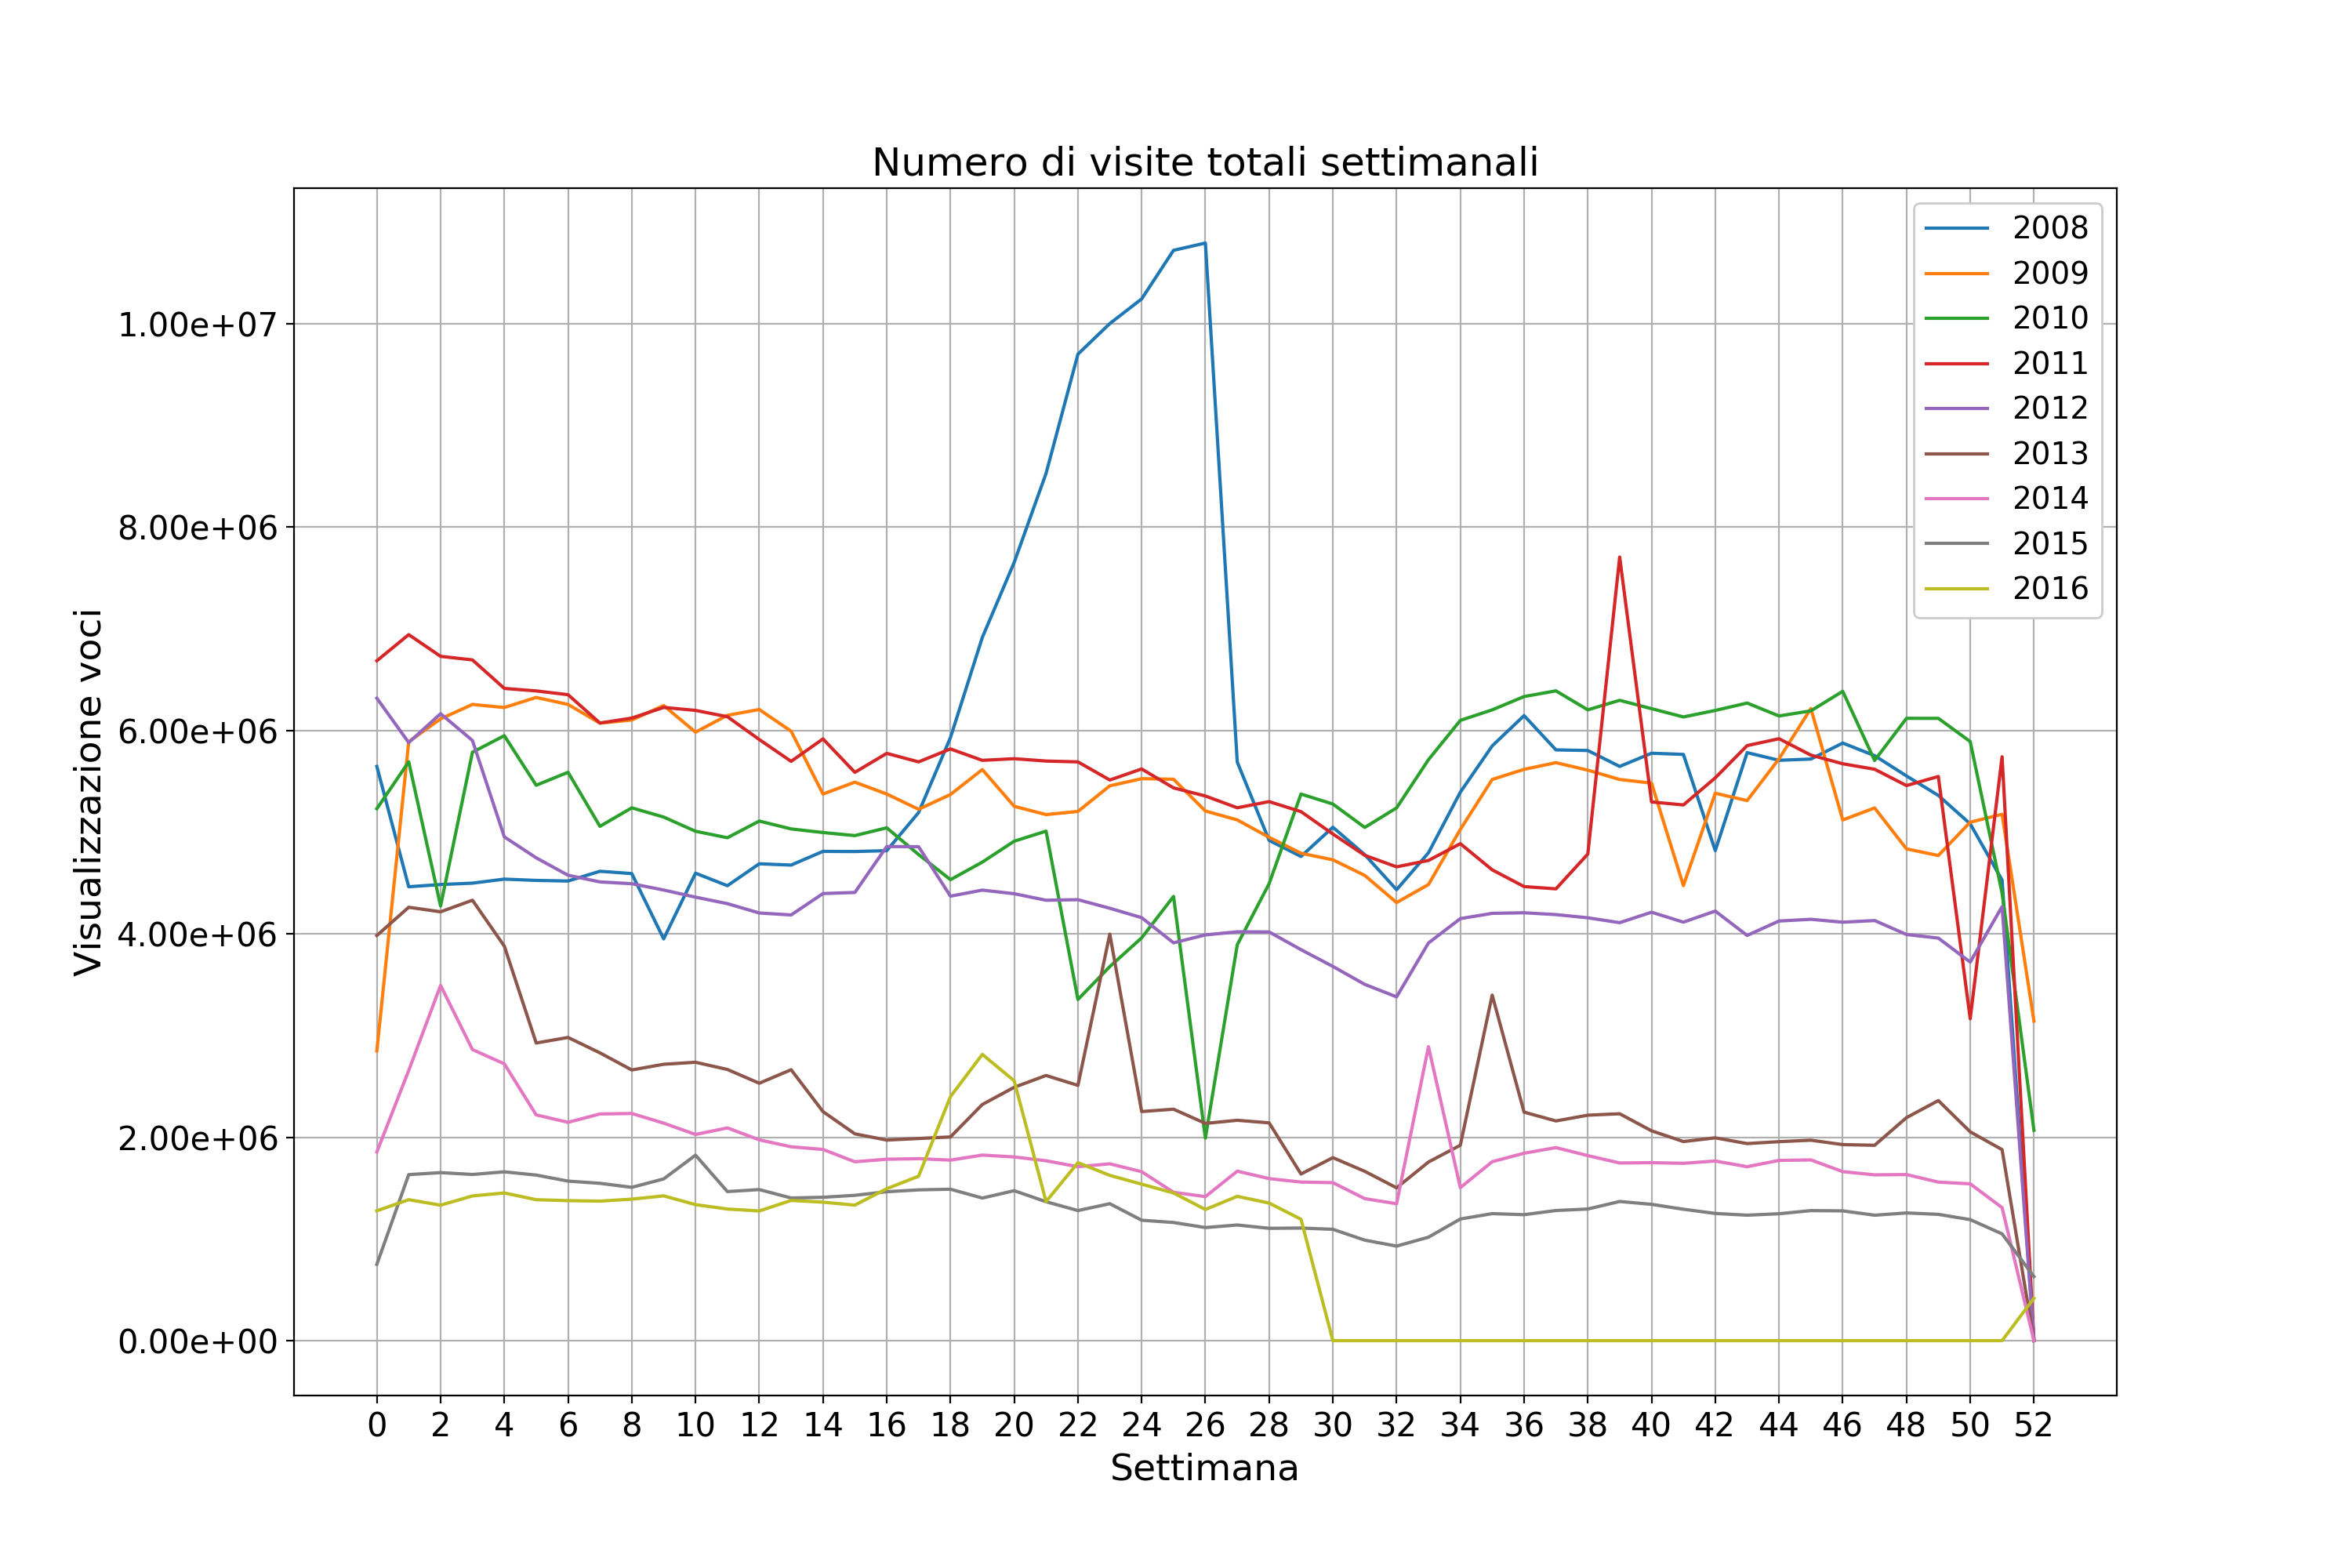
\includegraphics[scale=0.5]{chapter_2_weekly_visit}
%\caption{}
%\label{fig:ch_2_weekly_visit}
%\end{figure}

%\begin{figure}[h]
%\centering
%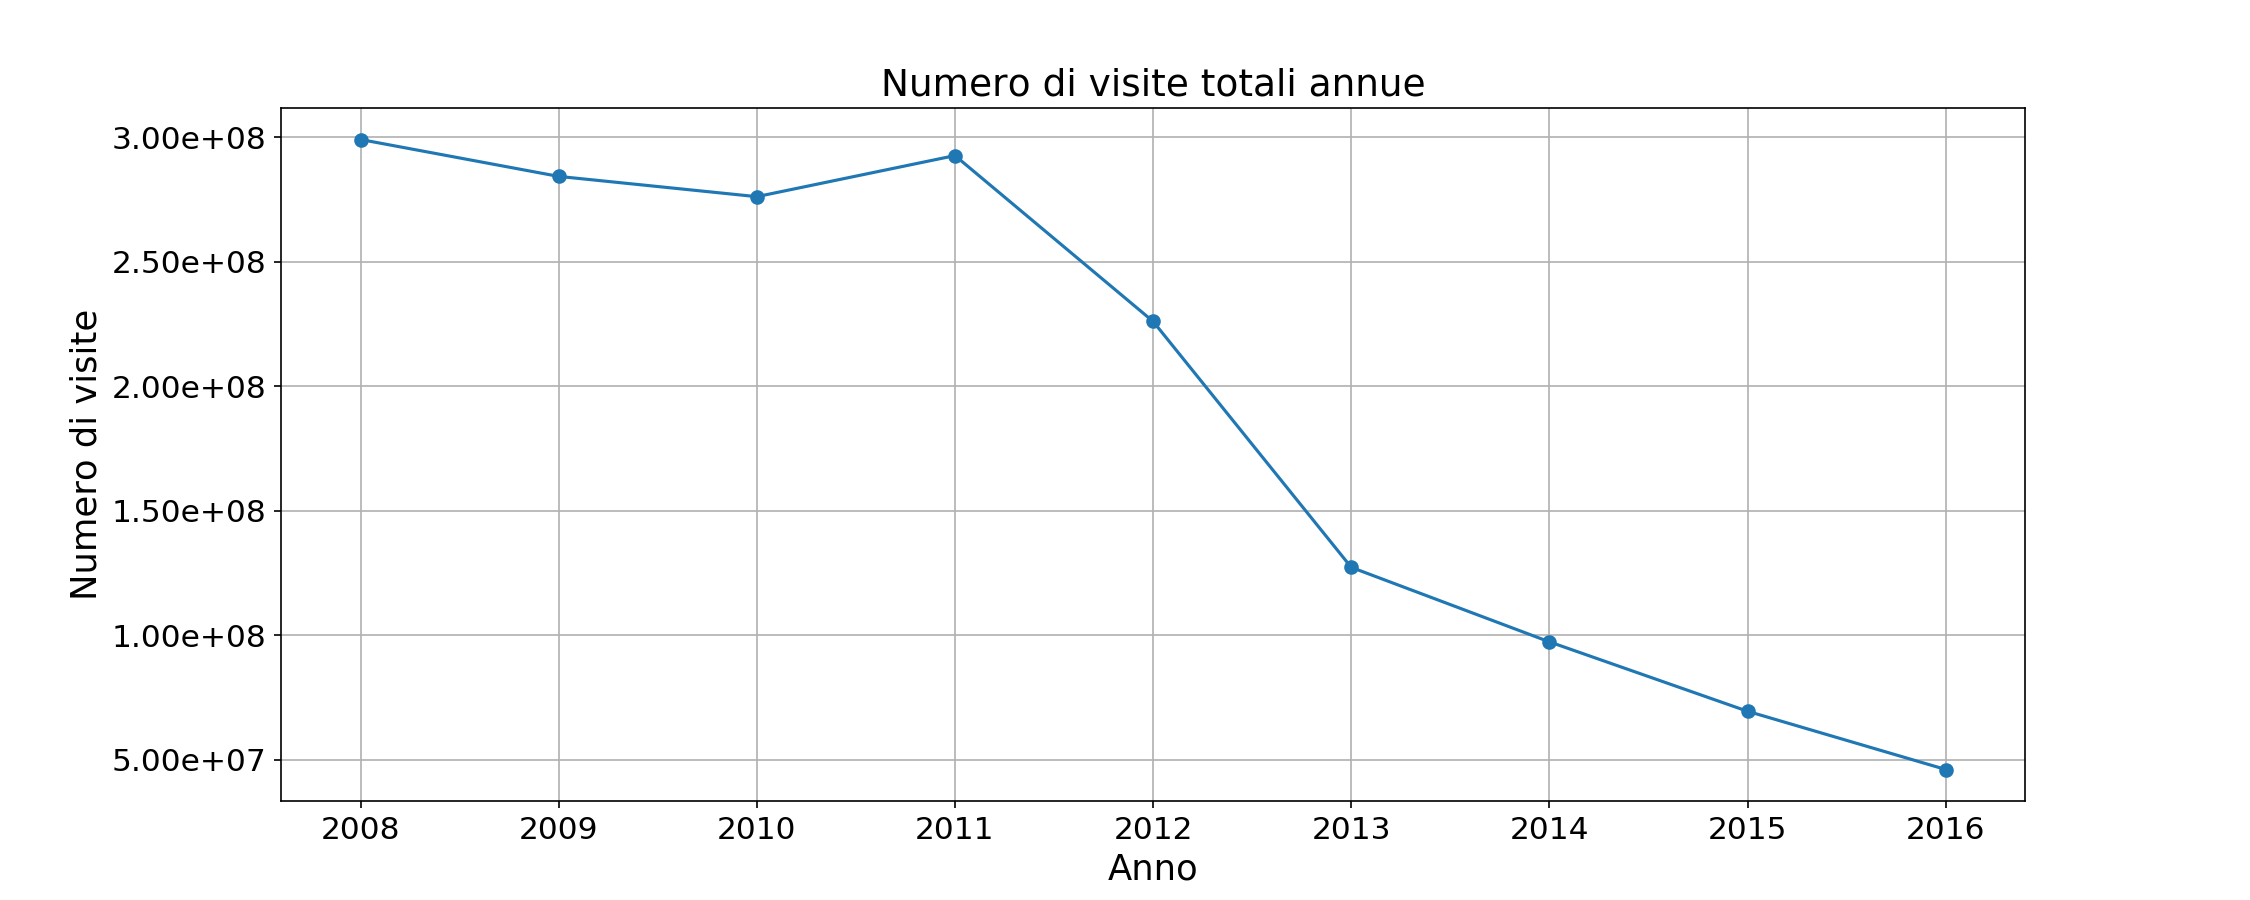
\includegraphics[scale=0.5]{chapter_2_annual_visit}
%\caption{}
%\label{fig:ch_2_annual_visit}
%\end{figure}


\end{document}
